\begin{abstract}

The human immune system is unexpectedly attentive towards
human transmembrane helices (TMHs), as TMH-derived peptide fragments
bind to histocompatibility complex (MHC) class I more often then expected
by chance only.
This finding hints that there has been selection upon detecting TMH-derived
peptides in pathogens.
If this signature of selection is present in MHC-II is unknown.
This study shows that MHC-I [also has/does not have] more
epitopes derived from a TMH for a pathogen proteome, when compared with
a host proteome.
Additionally, MHC-II binds to peptides derived from TMHs 
[less/equally/more] often than expected by chance.
Lastly, using an innovative computation method, 
we show that natural selection on TMHs is [strong enough/still too weak]
to detect.
Our findings suggest that the immune system is [less/neutral/more]
vigilant to TMHs than expected by chance and this has 
left [a clear/a weak/no]
signal in the evolutionary history of the pathogen.

\end{abstract}

{\bf Keywords:} antigen presentation, membrane proteins, bioinformatics, 
adaptive immunity, transmembrane domain, transmembrane helix, 
epitopes, T lymphocyte, MHC-1, MHC-I, MHC-2, MHC-II, COVID-19

%%%%%%%%%%%%%%%%%%%%%%%%%%%%%%%%%%%%%%%%%%%%%%%%%%%%%%%%%%%%%%%%%%%%%%%%%%%%%%%%
\section{Introduction}
%%%%%%%%%%%%%%%%%%%%%%%%%%%%%%%%%%%%%%%%%%%%%%%%%%%%%%%%%%%%%%%%%%%%%%%%%%%%%%%%

\paragraph{Immune response}

Our immune system fights invaders on a daily basis.
These invaders can be fungi, bacteria or viruses.
The innate immune response is its first general 
and immediate strategy, where the acquired immune response
needs time to develop its specialized and more effective
combat forces.

\paragraph{Immune response by MHC-I}

All nucleated cells in humans present randomly sampled peptides
fragments to the surroundings of the cell using the Major 
Histocompatibility Complex (MHC) class I molecules.
If a cell gets infected by a virus, also the virus' peptides
will be presented at the cell surface. The foreign viral antigen is detected 
by cytotoxic T lymphocytes, which will kill the infected cell.

\paragraph{Immune response by MHC-II}

All pathogens can be detected by the foreign proteins on 
their (bacterial or fungal) cell walls or (viral) envelope.
For bacteria and fungi, this is the main mode of their detection,
as these do not infect a cell with their (foreign) DNA.
T and B cells express MHC-II to detect foreign peptide fragments.
An immune response is started when MHC-II detects a pathogen.

\paragraph{Classification of HLA}

Any human's immune system detects only a fraction of all possible
peptide fragments.
For humans, the MHC proteins are encoded by the
HLA ('Human Leukocyte Antigens') genes.
Each MHC complex can only bind a subset of all possible peptides.
For example, HLA-A and HLA-B have no overlap in which
peptides they bind (\cite{lund2004definition}).
The HLA region of humans is highly polymorphic, 
making it hard to classify all of the many haplotypes.
Classification of HLAs is based on algorithms that
maximize the information content of each 
classification, such as the presence of a certain amino acid at 
the first (for MHC-II, \cite{southwood1998several})
or second position (for MHC-I, \cite{lund2004definition}) of a peptide.
However, this does not imply that when a peptide follows
a classification pattern, that it will bind to the MHC. 
Instead, software should be used to predict if the
full peptide will do so.

\paragraph{Epitope prediction}

It is helpful to be able to predict which peptides are immunogenic,
in, among others, vaccine development \richel{Reference here}. 
Already for a decade, synthesized peptide fragments are used
to experimentally determine which peptides
are immunogenic \richel{Reference here}.
This approach, however, is tedious and costly.
Due to this, software was written that allows for silico 
predictions, which are reliable in 
practice \cite{larsen2010identification,schellens2008unanticipated,tang2011genome}.
 
\paragraph{TMHs}

Transmembrane helices are conserved structures that span
a cell membrane with an alpha helix.
TMHs are hydrophobic, as this is required to span the 
hydrophobic cellular lipid membrane. Additionally,
they often have a length of 23 amino acids to be able to span
the membrane.
Polypeptide fragments derived from TMHs are among the most hydrophobic,
together with the internals of soluble proteins, where the
hydrophobicity parts guide the protein to achieve its 3D configuration.
TMHs are general structures: 25 percent of the human proteome is
anchored by at least one TMH. COVID-19 has 21 TMHs, 
making up for \richel{?} percent of its entire genome.
There are multiple computational tools developed to predict which
parts of membrane proteins are TMH.

\paragraph{MHC-I presents hydrophobic regions more often}

One might expect that the hydrophobic epitopes presented,
for a same hydrophobicity, are as likely to stem from 
membrane proteins TMHs or from soluble proteins hydrophobic (non-TMH) regions.
For MHC-I, however, it is found that the 9-mers stemming
from TMHs are presented more often than expected by 
chance \cite{bianchi2017}
\richel{but also when compensating for hydrophobicity?}.
For MHC-II, it is unknown which percentage of binders 
is derived from TMHs for all 13-mers present in a proteome
that have the same hydrophobicity.

\paragraph{HLAs increase detection range}

An increased detection
is obtained by expressing a wide variety of
MHCs, which is assured by the human leukocyte antigen gene complex (HLA).
However, a different HLA will result in a different variety of MHCs,
that will display different peptide fragments. Additionally, there
may have been selection the HLA to display and or detect different
peptide fragments.

\paragraph{MHC-I presents TMH-derived epitopes in humans more often}

For MHC-I, it was found that predicted epitopes derived 
from human transmembrane helices (TMHs)
are over-presented by all 5 HLA-A and 
most of 8 HLA-B super types (\cite{bianchi2017}).
One explanation is that the presentation of TMHs 
may have an evolutionary advantage for 
the (human) host, as TMHs have a reduced variability 
due to the functional requirement of being able to span a lipid bilayer. 
Due to this, pathogens have a lower chance to develop an escape mutation,
as many mutations will result in a dysfunctional TMH.
Note that the mechanism by which a cell presents its TMHs is
yet unknown.

\paragraph{Does MHC-I present TMH-derived epitopes from pathogens as often?}

It is important that MHC-I presents both the peptides of the 
(healthy) cell, as well as possible pathogen-derived peptides when the
cell is infected. As described above, MHC-I presents TMH-derived epitopes 
from the human host more often. It is unknown if MHC-I has the same
dedication to present epitopes that stem from TMHs derived from
proteins produced by pathogen, either would the pathogen
be a virus \richel{$\mathcal{H}_{1,1}$} or 
a bacterium \richel{$\mathcal{H}_{1,2}$}.

\paragraph{MHC-II is expected to present TMHs}

If presentation of TMHs on MHC-I would bring an evolutionary advantage 
in the recognition of pathogens by the immune system, 
it would follow that this is equally important for MHC-II, 
especially as the help of CD4+ T cells is needed for a long lasting CD8+ T cell 
response (\cite{novy2007cd4}). 
The mechanism to detect foreign TMHs by MHC-II would be unknown, 
similar to the discovery that MHC-I presents TMHs.

\paragraph{Does MHC-II present TMH-derived epitopes from pathogens as often?}

It is unknown if MHC-II, like MHC-I, 
presents TMH-derived epitopes as often, either 
in humans \richel{$\mathcal{H}_{2,1}$},
bacteria \richel{$\mathcal{H}_{2,2}$}
or viruses \richel{$\mathcal{H}_{2,3}$}.

\paragraph{Selection undetectable in whole proteome}

The human immune system and human pathogen are in an evolutionary
arms race: our immune systems is selected for the detection
of pathogens, whereas pathogens are selected to avoid detection.
From a pathogen's point of view, however, this struggle 
is of only minor importance:
in seasonal influenza, for example, the selection pressure
exerted by the immune system was only limited (\cite{han2019individual}).

In general, on would hope that evolutionary selection results in
an immune system that as most attentive for loci that are
essential for a virus, as these will be most conserved.
In COVID-19, for example, there is preliminary evidence that the strongest
selection pressure is upon residues that changes its 
virulence \cite{velazquez2020positive}.
These loci, however, only account for a small part of a pathogen's proteome.
Additionally, these essential parts differ widely between pathogens.
Because of this scarcity and variance in targets, 
one can imagine that the human immune system 
is not tailored to detect these sites, 
as hinted by upon by the aforementioned influenza study.

\paragraph{Selection may be detectable in TMHs}

TMHs, on the other hand, also have their function constraints, 
yet can occur multiple time a pathogen's proteome.
One can safely assume a pathogen's proteome contains multiple TMHs.
Therefore, it may be beneficial for the host
if its immune system would be more attentive towards TMHs.
And maybe this has already happened: MHC-I already detects hydrophobic
peptides. This feature, however, may also be caused by selection
to detect hydrophobic regions in the soluble proteins of pathogens.
It is unknown, when focusing on TMHs only, if a signal of selection
can be detected.

\paragraph{Selection needs to be additive}

Would a pathogen have only peptides that do not bind to
any HLA, a pathogen would be undetected. In that case, one
can imagine that a mutation
that causes a pathogen to become detected by a host's immune
system, may be selected against. Also, would a pathogen have only
one epitope, one can imagine there would be selection for a mutation to lose it.
If there are, however, already many epitopes present in the
proteome, the selection to lose or gain an epitope is expected 
to have less or no effect.

\paragraph{Immunodominance}

The effective number of epitopes, however,
is much lower than the actual number of possible
epitopes, due to immunodominance. 
Immunodominance is a feature of the immune system,
due to which some epitopes dominate in causing an immune response,
where other (called subdominant) epitopes end up having no 
effect \cite{akram2012immunodominance}.
The same study mentions 20 factors that influence the strength
of an immune response.
The most relevant factor for this study is the effect of
a mutation within an epitope, 
such as the in vitro example described in \cite{berkhoff2004mutation},
where one single mutation resulted in a 5-20\% weaker
response of virus-specific CD8+ T cells \richel{Fun experiment:
do this in silico}.
Due to immunodominance, we dare assume that there can be selection
for immune system avoidance, as the effective number of loci may be
low and effects of a single mutation noticeable.

\paragraph{Use of protein data in phylogenetics}

When using DNA sequences, one can use a skewed rate 
in non- versus synonymous mutation
to detect the signature of selection \cite{murrell2015gene}.
Using AA sequences, however, has its advantages,
as its is closer to the actual phenotype
selection acts upon: DNA may never be translated to RNA,
or its RNA may never be transcribed \cite{diz2012proteomics}
\richel{improve upon this point}.
When using a proteome in phylogenetic research,
we know that the majority of proteins are selected to just 
maintain their function most of the time, where
is the time spans there is selection, only a few AAs
can actually increase the 'fitness' of the 
protein \cite{anisimova2009investigating}.
There, when generalizing the dynamics of mostly purifying selection (to maintain
a protein's function) and a short duration of positive selection,
those genes that are selected cannot be detected \cite{yang2000statistical}.

\paragraph{Evolutionary signal of unknown strength for pathogens}

Up until today, it is unknown if an evolutionary signal 
is present in a (human) pathogen's proteome that stems from avoiding
detection by the human immune system.
If such a signal is present, we expect to detect it most likely in
viruses, as both MHC-I and MHC-II are used in protecting the
human host. 
Therefore, this study focuses in detecting this signal in viruses.

%%%%%%%%%%%%%%%%%%%%%%%%%%%%%%%%%%%%%%%%%%%%%%%%%%%%%%%%%%%%%%%%%%%%%%%%%%%%%%%%
\section{Hypotheses}
%%%%%%%%%%%%%%%%%%%%%%%%%%%%%%%%%%%%%%%%%%%%%%%%%%%%%%%%%%%%%%%%%%%%%%%%%%%%%%%%

\richel{Will be moved to supplementary materials}

\begin{itemize}
  \item $\mathcal{H}_{1,VB}$: MHC-I has the same percentage of epitopes overlapping
    with viral/bacterial TMHs as with human TMHs
  \item $\mathcal{H}_{2,HVB}$: MHC-II has the same percentage of epitopes overlapping
    with human/viral/bacterial TMHs as expected by chance
  \item $\mathcal{H}_{3}$: The mutations observed in 
    viral TMHs are caused by chance.
    Alternatively, these are caused by natural selection
    induced by (non-)binding to HLAs
\end{itemize}

%%%%%%%%%%%%%%%%%%%%%%%%%%%%%%%%%%%%%%%%%%%%%%%%%%%%%%%%%%%%%%%%%%%%%%%%%%%%%%%%
\section{Methods}
%%%%%%%%%%%%%%%%%%%%%%%%%%%%%%%%%%%%%%%%%%%%%%%%%%%%%%%%%%%%%%%%%%%%%%%%%%%%%%%%

\paragraph{Data sets for TMH epitopes}

To determine the percentages of epitopes overlapping
with TMHs, we use three reference proteomes, which are
a human, viral and bacterial one.
The human reference proteome is \richel{here}, 
which is the same as \cite{bianchi2017}.
The viral reference proteome is represented by
the proteome of the first sequenced COVID-19 strain (\cite{wu2020new},
GenBank ID of MN908947.3, \url{https://www.ncbi.nlm.nih.gov/nuccore/MN908947})
For bacteria, the reference genome of 
Mycobacterium tuberculosis (\url{https://www.ebi.ac.uk/reference_proteomes}, UP000001584, 
83332 MYCTU) is used.

\paragraph{Data set for evolutionary selection}

To detect an evolutionary signal for selection on binding
TMHs peptides, we need a phylogenetic tree with 
many time-dated proteomes.
To do so, we use a viral pathogen, as these are detected by both
MHC-I and MHC-II.
To detect individual mutations, we need a high resolution dataset
that also includes the evolutionary history of the virus.
COVID-19 satisfies both requirements:
as of 2020-06-22, it has 49790 proteomes, as provided by GISAID (\cite{shu2017gisaid}),
as well as a provided evolutionary history by Nextstrain (\cite{hadfield2018nextstrain}).

%%%%%%%%%%%%%%%%%%%%%%%%%%%%%%%%%%%%%%%%%%%%%%%%%%%%%%%%%%%%%%%%%%%%%%%%%%%%%%%%
\subsection{Measuring TMH epitopes}
%%%%%%%%%%%%%%%%%%%%%%%%%%%%%%%%%%%%%%%%%%%%%%%%%%%%%%%%%%%%%%%%%%%%%%%%%%%%%%%%

To determine the percentages of MHC-I and MHC-II epitopes overlap
with TMHs, we used mostly the same analysis as described in \cite{bianchi2017}.
To summarize: a proteome is converted into all its possible 9-mers. For each
of these peptides, it is measured if it has been part of a TMH (at least
1 residue), as well as if the peptide is a binder to an MHC-I haplotype.
Because the percentage of TMH residues is known, a binomial test can be
used to determine if TMH-derived peptides are as likely to be a binder
as expected by chance (the null hypothesis), or that TMHs are indeed an
overrepresented source of epitopes (as found by \cite{bianchi2017}).

This study differs in some aspects, described below in more detail,
which is the definition of what a binder is,
the addition of using MHC-II haplotypes, the software used,
and the significance level to determine if TMH-derived peptides are as 
likely to be a binder as expected by chance.
These deviations are either a refinement of the previous method or
a pragmatic choice made due to the extension of the original experiment.

The definition of a binder differs from \cite{bianchi2017}:
in this study a peptide is labeled an MHC-I binder if, within a haplotype, 
any of its 9-mer peptides have an IC50 in the lowest 2\% of randomly simulated 
peptides (see table \ref{table:ic50s_per_haplotype} for values), were the original study defined
a binder as having an IC50 in the lowest 2\% of the peptides within a protein.
% See https://github.com/richelbilderbeek/bianchi_et_al_2017/blob/72e6755a31d400158368509fd80a41e984677ab1/predict-binders.R#L17

The 13 MHC-I haplotypes used in this study are the same as 
the ones in \cite{bianchi2017}.
The MHC-II haplotypes used additionally are selected 
to occur with a phenotypic frequency of at least 14\% in
the human population (\cite{greenbaum2011functional},
see \ref{table:mhc2_haplotypes} for coverage),
resulting in 13 haplotypes.
This frequency threshold is arbitrarily chosen to result in 
the same number of haplotypes for each MHC class
\richel{Add this to bbbq, there it is now 21}.
When using an MHC-II haplotype, instead of using 9-mers, 13-mers are
used, as these are the canonical MHC-II epitope size \richel{Reference here}.

Instead of using the MHC-I-only epitope prediction 
tool \verb;EpitopePrediction;, MHCnuggets is used, as it can predict
both MHC-I and MHC-II epitopes.
Additionally, instead of only using a human proteome, in this study
also a viral and bacterial proteome are analyzed.

Where the original study used a significance level of 1\% 
for the binomial test to determine if TMH-derived peptides 
are as likely to be a binder as expected by chance, this study
uses 5\%, which is a common significance level for an exploratory study.

%%%%%%%%%%%%%%%%%%%%%%%%%%%%%%%%%%%%%%%%%%%%%%%%%%%%%%%%%%%%%%%%%%%%%%%%%%%%%%%%
\subsection{Comparing amounts of TMH epitopes}
%%%%%%%%%%%%%%%%%%%%%%%%%%%%%%%%%%%%%%%%%%%%%%%%%%%%%%%%%%%%%%%%%%%%%%%%%%%%%%%%

To determine if MHC-I has the same percentage of epitopes overlapping
with viral/bacterial TMHs as with human TMHs \richel{$\mathcal{H}_{1,VB}$}, 
we compare the distributions of the measured percentages 
of TMH-overlapping peptides for all haplotypes,
and compare the distributions between humans and each pathogen
using a two-sample Kolmogorov-Smirnov (KS) test
for a significance level $\alpha = 0.05$, 
which is a common significance level for an exploratory study.

%%%%%%%%%%%%%%%%%%%%%%%%%%%%%%%%%%%%%%%%%%%%%%%%%%%%%%%%%%%%%%%%%%%%%%%%%%%%%%%%
\subsubsection{Detecting evolution}
%%%%%%%%%%%%%%%%%%%%%%%%%%%%%%%%%%%%%%%%%%%%%%%%%%%%%%%%%%%%%%%%%%%%%%%%%%%%%%%%

\paragraph{Introduction}

To detect evolution, we determine the probability 
that all of the observed TMH mutations have arisen by chance,
with regards to being detected/presented by the immune system,
per MHC class and haplotype. We do this for human, viral and
bacterial TMHs.

\paragraph{Correction against many tests}

% Chance to find
%            this amount of positives (sums to 1)
%              |
%              v
% > dbinom(x = 0, size = 26, prob = 0.05)
% [1] 0.2635201
% > dbinom(x = 1, size = 26, prob = 0.05)
% [1] 0.3606064
% > dbinom(x = 2, size = 26, prob = 0.05)
% [1] 0.2372411
% > dbinom(x = 3, size = 26, prob = 0.05)
% [1] 0.09989098
% > dbinom(x = 4, size = 26, prob = 0.05)
% [1] 0.03023017
% > dbinom(x = 5, size = 26, prob = 0.05)
% [1] 0.00700067
%
% Chance to find more than
%            this amount of positives (excluding the value!)
%              |
%              v
% > pbinom(q = 0, size = 26, prob = 0.05, lower.tail = FALSE)
% [1] 0.7364799
% > pbinom(q = 1, size = 26, prob = 0.05, lower.tail = FALSE)
% [1] 0.3758735
% > pbinom(q = 2, size = 26, prob = 0.05, lower.tail = FALSE)
% [1] 0.1386324
% > pbinom(q = 3, size = 26, prob = 0.05, lower.tail = FALSE)
% [1] 0.0387414
% > pbinom(q = 4, size = 26, prob = 0.05, lower.tail = FALSE)
% [1] 0.008511231


Because we use 13 haplotypes per MHC class,
for a significance level of 5\%,
for both directions (D to U, or U to D)
we expect 5% times 26 equals 1.3 significant findings.

\richel{Hmm, improve}
The chance to find 2 haplotypes that hint to have selection working upon it
is 4\%, which is below our significance level.
% > pbinom(q = 3, size = 26, prob = 0.05, lower.tail = FALSE)
% [1] 0.0387414

Upon finding 3 haplotypes that hint to have selection working upon it,
there is the additional chance that selection is working in different
directions (i.e. in one case there is selection for losing detection,
where in the other case, there is (unexpected) selection for gaining
detection). Therefore, finding 3 haplotypes that hint to have selection working 
upon it in the same direction 

Therefore, we will claim there is directional selection, 
when, for a proteome, we find 2 haplotypes 
that hint to have selection working upon it

\paragraph{System depicted as a Markov chain}
 
To calculate the probability all of our observations happened by chance,
we view our experiment as a two-state Markov chain, as depicted in
figure \ref{fig:markov_chain}. The two nodes depict the
two possible detection state a peptide is in, which is
either undetected $U$, or detected $D$ by the immune system,
where a detected peptide is a binder, that is, 
a peptide with an IC50 in the lowest 2\%.
The $D$ can be either detection by an MHC-I or MHC-II haplotype.
The edges depict the probability of a state transition by mutation,
for example, $p_{DU}$ denotes the probability that a detected
peptide mutates into an undetected one.
We focus on peptides that are TMH and we assume a mutation that 
renders the TMH non-functional as lethal.

\begin{figure}
  \centering
  \input{markov_chain_2_states.latex}
  \caption{
    State transitions in TMHs caused by mutations, with respect to the
    detection by the immune system. Any TMH is either in a detected, $D$, or
    undetected, $U$, state. Mutations cause state transitions with probability
    $p$. For example, $p_{DU}$ denotes the probability that a detected
    TMH mutates into an undetected one.
  }
  \label{fig:markov_chain}
\end{figure}

\paragraph{Statistics}

When we have calculated the probability of each transition (as described below),
we can simply count the number of observed transitions.
Because the probability of transitions differ per peptide,
the total system has the properties of a Poisson binomial distribution,
from which we can calculate the probability of the observing our
number of transitions.

\paragraph{Hypotheses testing}

Of the complete system, we test for each of the 2 observed 
state transition rates (that is, we do not test for mutations that result in the same state)
if these are likely to be caused by chance.
For each transition rate, we know the expected and observed number
of transitions. If the observed number of transitions is below the expected
value, we test for finding that (low) number of transitions or less.
If the observed number of transitions is above the expected
value, we test for finding that (high) number of transitions or more.
We use a significance level $\alpha$ of 5\%, because we have no prior
expectations. 

As we are testing 2 rates (and thus 2 hypotheses), 
we correct against type I errors (false positives), 
by applying the Bonferroni correction, 
resulting in $\alpha_c = \frac{\alpha}{2}$.
If the probability of observing that few/many 
transition is below $\alpha_c$, we will state 
that this unlikely situation may be caused by natural selection.

\paragraph{Calculating one peptide's probability}

We calculate the probability of a transition per peptide.
For any peptide, we can generate all sequences that differ
in only one amino acids. Of these sequences, we only keep the ones
that result in a TMH. Of each of the remaining TMH sequences, we predict
which mutants are detected by the immune system. Because not all 
AA mutations are equally likely, we correct for the AA transition
rates using the FLU transition matrix (\cite{dang2010flu}),
which is a transition matrix derived from observed influenza AA mutations.

\paragraph{Assumption that epitopes are immunogenic}

We assume that if a peptide binds to an MHC, it is always presented and always
leads to an immune response.
The more often this assumption is violated, 
the more our analysis will be weakened.
Experiments in mice with MHC-I epitopes, however, indicate that (if the dose 
administered was high enough) there are either none or rare
exceptions \cite{sette1994relationship}.

\paragraph{Measuring strength}

To assess the strength of our analysis, 
we have applied it to four simulated data sets,
which are the product of using either MHC-I or MHC-II,
as well as using two different selection scenarios.

For both MHC-I and MHC-II, we use the haplotypes that have 
the lowest phenotypic frequency, which is \richel{X} for MHC-I
and DPB1*0501 (21.7\%) for MHC-II.

The two selection scenarios are either no selection
or a two-fold selection on what we would expect.
The scenario without selection, the 'null' data set, acts 
as a control, where we let the simulate observations occur by chance. 
The 'rigged' data set is a data set in which we 
let evolution bias the observations two-fold, that is, 
we let mutations that are beneficial occur twice as often as expected by chance.

All data sets consists out of $10^4$ observations.
Each observation starts with a randomly generated source peptide fragment,
as well a mutant. For the 'null' data set, the mutant is randomly select.
For the 'rigged' data set, beneficial mutations are twice as likely to
be selected. We define a beneficial mutation as a transition from
being detected to being undetected.

%%%%%%%%%%%%%%%%%%%%%%%%%%%%%%%%%%%%%%%%%%%%%%%%%%%%%%%%%%%%%%%%%%%%%%%%%%%%%%%%
\subsection{Prediction software used}
%%%%%%%%%%%%%%%%%%%%%%%%%%%%%%%%%%%%%%%%%%%%%%%%%%%%%%%%%%%%%%%%%%%%%%%%%%%%%%%%

For this research, the scientific literature was explored 
to find the most recent free and open source (FOSS) prediction software.
This was done by searching for papers that (1) reference older
prediction software, and (2) present a novel method to make predictions.
As a starting point, a review paper was used.

\paragraph{TMH prediction}

There are multiple computational tools developed to predict which
parts of membrane proteins are TMH
In 2001, multiple tools to do so have been compared \cite{moller2001evaluation},
of which TMHMM \cite{krogh2001predicting} turned out to be the best, yet
this software has a restrictive software license and is nearly two
decades old. Inspired on TMHMM, many other tools followed, such as 
Phobius (\cite{kall2004combined}),
ConPred II (\cite{arai2004conpred}),
MEMSAT3 (\cite{jones2007improving})
and MetaTM (\cite{klammer2009metatm}).
The most recent FOSS tool is called PureseqTM (\cite{wang2019efficient}),
which is used in this study.

\paragraph{MHC-I epitope prediction}

For MHC-I, there are multiple computational tools developed 
to predict epitopes. 
According to \cite{lundegaard2011prediction}, in 2011,
from a set of multiple tools, 
NetMHCcons \cite{karosiene2012netmhccons} gave the best predictions.
A tool developed later is \verb;epitope-prediction; \cite{bianchi2017},
which uses a stabilized matrix method \cite{kim2009derivation}.
The most recent FOSS tool available is MHCnuggets\cite{shao2020high},
which we will use in this study

\paragraph{MHC-II epitope prediction}

Also for MHC-II, there are multiple computational tools developed 
to predict epitopes,
such as using a trained neural network (\cite{nielsen2003reliable})
or a Gibbs sampling approach (\cite{nielsen2004improved}).
According to \cite{lundegaard2011prediction}, in 2011,
from a set of multiple tools, 
NetMHCIIpan (\cite{nielsen2008quantitative,karosiene2013netmhciipan})
gave rise to the most accurate predictions.
Later tools are \cite{zhang2013predicting},
\cite{trolle2014nettepi}, \cite{zhang2015accurate}
and the very recent MHCnuggets (\cite{shao2020high}),
the latter which we will use in this study.

% \paragraph{Gene prediction}
% 
% Proteogenomics is the field dedicated to, among others,
% predict the proteins that arise from a DNA 
% sequence \cite{nesvizhskii2014proteogenomics}.
% For an ab initio gene prediction of a viral genome, 
% we searched the literature for the most recent software tool,
% which is Vgas (\cite{zhang2019vgas}). In this article, 
% Vgas is compared to tools, such as GeneMarkS (\cite{besemer2001genemarks}),
% Prodigal (\cite{hyatt2012gene}), GLIMMER (\cite{delcher1999improved}),
% RAST \cite{aziz2008rast} and prokka (\cite{seemann2014prokka}).
% We picked the FOSS tool that scored best in the (closed source) Vgas
% benchmark (\cite{zhang2019vgas}), which is Prodigal.

%%%%%%%%%%%%%%%%%%%%%%%%%%%%%%%%%%%%%%%%%%%%%%%%%%%%%%%%%%%%%%%%%%%%%%%%%%%%%%%%
\subsection{Prediction software written}
%%%%%%%%%%%%%%%%%%%%%%%%%%%%%%%%%%%%%%%%%%%%%%%%%%%%%%%%%%%%%%%%%%%%%%%%%%%%%%%%

The R programming language is used for the complete 
experiment, including the analysis.
The complete experiment is bundled in the 'bbbq' R package,
which is dependent on 'pureseqtmr', 'mhcnuggetsr' and 'mhcnpreds',
as described below.

To be able to call, from R, the TMH prediction software 'PureseqTM',
which is written in C, the package 'pureseqtmr' has been developed. 
'pureseqtmr' allows to install 'PureseqTM' and use most of its features.
Excluded are the features that are used by the 'PureseqTM' 
developers to verify the correctness of their work.
'pureseqtmr' has been submitted to CRAN.

The R package 'mhcnuggetsr' is written to call the 
'MHCnuggets' Python package.
'mhcnuggetsr' allows to install 'MHCnuggets' and call it
to predict IC50 values for multiple MHC haplotypes that 'MHCnuggets' 
has already been trained upon.
Excluded is the feature to train 'MHCnuggets' on new data and/or other
haplotypes, as this study only needs IC50 predictions.
'mhcnuggetsr' has been submitted to CRAN.

To be able to use pre-calculated MHCnuggets
predictions (i.e. a distribution of IC50 values per haplotype, 
derived from random peptides), the 'mhcnpreds' R package has been 
developed. In practice, this is nothing more than a big look-up table.
Because the package is too big, it will not been submitted to CRAN.

To reproduce the full experiment as done in this paper,
the functions needed are bundled in the 'bbbq' R package.
This package is too specific to be submitted to CRAN.

%%%%%%%%%%%%%%%%%%%%%%%%%%%%%%%%%%%%%%%%%%%%%%%%%%%%%%%%%%%%%%%%%%%%%%%%%%%%%%%%
\section{Results}
%%%%%%%%%%%%%%%%%%%%%%%%%%%%%%%%%%%%%%%%%%%%%%%%%%%%%%%%%%%%%%%%%%%%%%%%%%%%%%%%

%%%%%%%%%%%%%%%%%%%%%%%%%%%%%%%%%%%%%%%%%%%%%%%%%%%%%%%%%%%%%%%%%%%%%%%%%%%%%%%%
\subsection{MHC-I}
%%%%%%%%%%%%%%%%%%%%%%%%%%%%%%%%%%%%%%%%%%%%%%%%%%%%%%%%%%%%%%%%%%%%%%%%%%%%%%%%

Figure \ref{fig:1} shows the percentages of MHC-I epitopes overlapping 
with TMHs for our human, viral and bacterial proteome.

The KS test to determine if MHC-I has the same percentage 
of epitopes overlapping with viral TMHs, 
compared to human TMHs \richel{$\mathcal{H}_{1,V}$},
resulted in a p-value of \richel{unknown},
which makes us [reject/accept] the hypothesis that these percentages
are sampled from the same distribution. 

The KS test to determine if MHC-I has the same percentage 
of epitopes overlapping with bacterial TMHs, 
compared to human TMHs \richel{$\mathcal{H}_{1,B}$},
resulted in a p-value of \richel{unknown},
which makes us [reject/accept] the hypothesis that these percentages
are sampled from the same distribution. 

\begin{figure}[!htbp]
  \includegraphics[width=\textwidth]{bbbq_1/fig_f_tmh_mhc1.png}
  \caption{
    Percentage of MHC-I epitopes overlapping with TMHs
    for a human, viral and bacterial proteome.
  }
  \label{fig:1}
\end{figure}

%%%%%%%%%%%%%%%%%%%%%%%%%%%%%%%%%%%%%%%%%%%%%%%%%%%%%%%%%%%%%%%%%%%%%%%%%%%%%%%%
\subsection{MHC-II}
%%%%%%%%%%%%%%%%%%%%%%%%%%%%%%%%%%%%%%%%%%%%%%%%%%%%%%%%%%%%%%%%%%%%%%%%%%%%%%%%

Figure \ref{fig:2} shows the percentages of MHC-II epitopes overlapping 
with TMHs for our human, viral and bacterial proteome.

\begin{figure}[!htbp]
  \includegraphics[width=\textwidth]{bbbq_1/fig_f_tmh_mhc2.png}
  \caption{
    \% epitopes overlapping with transmembrane helix
    for a human, COVID-19 and Mycobacterium proteome.
  }
  \label{fig:2}
\end{figure}

%%%%%%%%%%%%%%%%%%%%%%%%%%%%%%%%%%%%%%%%%%%%%%%%%%%%%%%%%%%%%%%%%%%%%%%%%%%%%%%%
\section{Conclusion}
%%%%%%%%%%%%%%%%%%%%%%%%%%%%%%%%%%%%%%%%%%%%%%%%%%%%%%%%%%%%%%%%%%%%%%%%%%%%%%%%

We found that the percentages of epitopes overlapping 
with TMHs for a human and viral proteome are 
[similar/different]. In other words, the
epitopes that MHC-I presents are [as/not as] likely 
to be derived from TMH within either a human host and its viral pathogen.

We found that the percentages of epitopes overlapping 
with TMHs for a human and bacterial proteome are 
[similar/different]. In other words, the
epitopes that MHC-I presents are [as/not as] likely 
to be derived from TMH within either a human host and its bacterial pathogen.

%%%%%%%%%%%%%%%%%%%%%%%%%%%%%%%%%%%%%%%%%%%%%%%%%%%%%%%%%%%%%%%%%%%%%%%%%%%%%%%%
\section{Discussion}
%%%%%%%%%%%%%%%%%%%%%%%%%%%%%%%%%%%%%%%%%%%%%%%%%%%%%%%%%%%%%%%%%%%%%%%%%%%%%%%%

We concluded that the
epitopes that MHC-I presents are [as/not as] likely 
to be derived from TMH within either a human host and its viral pathogen.
Because the full COVID-19 has 21 TMHs, the percentages
of MHC-I epitopes being part of a TMH are likelier to be affected by
stochasticity. We chose to use COVID-19 regardless, as the thousands
of its time-dated genomic sequences are ideal for determining the 
evolutionary conservation of MHC-I detecting TMHs. 

We concluded that the
epitopes that MHC-I presents are [as/not as] likely 
to be derived from TMH within either a human host and its bacterial pathogen.
Because a bacterium does not infect a cell, thus its peptides
will not be presented by MHC-I, this result is [unexpected/expected]

We aimed our evolutionary experiment at TMHs, because these can
be predicted well from a protein structure,
are common structures and are present in all pathogens. 
We could have done the same experiment on beta-turn,
as also these can be predicted well \cite{petersen2010netturnp},
are common structures and are present in all pathogens.

\richel{
  Note that most bacteria are opportunistic pathogens.
  Note that most bacteria are generalists.
  Note that most bacteria have different cell membranes (and walls), that
  may have different functional constraints than a human cell membrane
}

%%%%%%%%%%%%%%%%%%%%%%%%%%%%%%%%%%%%%%%%%%%%%%%%%%%%%%%%%%%%%%%%%%%%%%%%%%%%%%%%
\section{Acknowledgments}
%%%%%%%%%%%%%%%%%%%%%%%%%%%%%%%%%%%%%%%%%%%%%%%%%%%%%%%%%%%%%%%%%%%%%%%%%%%%%%%%

We thank the Center for Information Technology of the University 
of Groningen for its support and for providing access to the Peregrine 
high performance computing cluster. 
Additionally, we would like to thank Sci-Hub \cite{himmelstein2018sci}
for allowing us to read paywalled articles while working from home.

%%%%%%%%%%%%%%%%%%%%%%%%%%%%%%%%%%%%%%%%%%%%%%%%%%%%%%%%%%%%%%%%%%%%%%%%%%%%%%%%
\section{Data Accessibility}
%%%%%%%%%%%%%%%%%%%%%%%%%%%%%%%%%%%%%%%%%%%%%%%%%%%%%%%%%%%%%%%%%%%%%%%%%%%%%%%%

All code is archived at \url{http://github.com/richelbilderbeek/someplace},
with DOI \url{https://doi.org/12.3456/zenodo.1234567}.

%%%%%%%%%%%%%%%%%%%%%%%%%%%%%%%%%%%%%%%%%%%%%%%%%%%%%%%%%%%%%%%%%%%%%%%%%%%%%%%%
\section{Authors' contributions}
%%%%%%%%%%%%%%%%%%%%%%%%%%%%%%%%%%%%%%%%%%%%%%%%%%%%%%%%%%%%%%%%%%%%%%%%%%%%%%%%

RJCB and FB conceived the idea for this research. 
RJCB wrote the code.
RJCB and FB wrote the article.

%%%%%%%%%%%%%%%%%%%%%%%%%%%%%%%%%%%%%%%%%%%%%%%%%%%%%%%%%%%%%%%%%%%%%%%%%%%%%%%%
% Bibliography
%%%%%%%%%%%%%%%%%%%%%%%%%%%%%%%%%%%%%%%%%%%%%%%%%%%%%%%%%%%%%%%%%%%%%%%%%%%%%%%%
% MEE style
\bibliographystyle{mee}
\bibliography{bbbq_article}
%%%%%%%%%%%%%%%%%%%%%%%%%%%%%%%%%%%%%%%%%%%%%%%%%%%%%%%%%%%%%%%%%%%%%%%%%%%%%%%%


%%%%%%%%%%%%%%%%%%%%%%%%%%%%%%%%%%%%%%%%%%%%%%%%%%%%%%%%%%%%%%%%%%%%%%%%%%%%%%%%
\appendix
\section{Supplementary materials}
%%%%%%%%%%%%%%%%%%%%%%%%%%%%%%%%%%%%%%%%%%%%%%%%%%%%%%%%%%%%%%%%%%%%%%%%%%%%%%%%

%%%%%%%%%%%%%%%%%%%%%%%%%%%%%%%%%%%%%%%%%%%%%%%%%%%%%%%%%%%%%%%%%%%%%%%%%%%%%%%%
\subsection{Differences with Bianchi et al., 2017}
%%%%%%%%%%%%%%%%%%%%%%%%%%%%%%%%%%%%%%%%%%%%%%%%%%%%%%%%%%%%%%%%%%%%%%%%%%%%%%%%

A part of this study does the same analysis as Bianchi et al., 2017.
Here we describe the deviations, which are about the use of different
software and the use of a different definition of what a binder is.

\paragraph{TMH prediction software}

The earlier study uses TMHMM, which has a restricted software license.
Instead, we chose to use PureseqTM, which is free and open source.

\paragraph{IC50 prediction software}

The earlier study uses a hand-crafted method, that only works on MHC-I.
Instead, we use MHCnuggets, which (1) free and open source, and (2) predicts
IC50s on both MHC-I and MHC-II.

\paragraph{Definition of what a binder is}

The earlier study defines a peptide a binder (for a haplotype), 
if \emp{within the peptide} in which it is found, 
is within the peptides with the 2\% lowest IC50 values.
This can be seen at \url{https://github.com/richelbilderbeek/bianchi_et_al_2017/blob/master/predict-binders.R},
where the binders are written to file.

In this study, a peptide is defined a binder (for a haplotype), 
if \emp{within a proteome} in which it is found, 
is within the peptides with the 2\% lowest IC50 values.

%%%%%%%%%%%%%%%%%%%%%%%%%%%%%%%%%%%%%%%%%%%%%%%%%%%%%%%%%%%%%%%%%%%%%%%%%%%%%%%%
\subsection{MHC-I}
%%%%%%%%%%%%%%%%%%%%%%%%%%%%%%%%%%%%%%%%%%%%%%%%%%%%%%%%%%%%%%%%%%%%%%%%%%%%%%%%

\input{bbbq_1/table_tmh_binders_mhc1.latex}

%\begin{table}[!htbp]
%   \input{bbbq_1/bbbq_1_stats_covid.latex}
%   \caption{
%     Kolmogorov-Smirnov test results comparing human and COVID-19 for MHC-I
%     \richel{Done on the simulated data}
%   }
%   \label{table:bbbq_1_stats_covid}
% \end{table}

% \begin{table}[!htbp]
%   \input{bbbq_1/bbbq_1_stats_myco.latex}
%   \caption{
%     Kolmogorov-Smirnov test results comparing human and Mycobacterium for MHC-I
%     \richel{Done on the simulated data}
%   }
%   \label{table:bbbq_1_stats_myco}
% \end{table}

%%%%%%%%%%%%%%%%%%%%%%%%%%%%%%%%%%%%%%%%%%%%%%%%%%%%%%%%%%%%%%%%%%%%%%%%%%%%%%%%
\subsection{MHC-II}
%%%%%%%%%%%%%%%%%%%%%%%%%%%%%%%%%%%%%%%%%%%%%%%%%%%%%%%%%%%%%%%%%%%%%%%%%%%%%%%%

\input{bbbq_1/table_tmh_binders_mhc2.latex}

% \begin{table}[!htbp]
%   \input{bbbq_2/bbbq_2_stats_covid.latex}
%   \caption{
%     Kolmogorov-Smirnov test results comparing human and COVID-19 for MHC-II
%     \richel{Done on the simulated data}
%   }
%   \label{table:bbbq_2_stats_covid}
% \end{table}

% \begin{table}[!htbp]
%   \input{bbbq_2/bbbq_2_stats_myco.latex}
%   \caption{
%     Kolmogorov-Smirnov test results comparing human and Mycobacterium for MHC-II
%     \richel{Done on the simulated data}
%   }
%   \label{table:bbbq_2_stats_myco}
% \end{table}


%%%%%%%%%%%%%%%%%%%%%%%%%%%%%%%%%%%%%%%%%%%%%%%%%%%%%%%%%%%%%%%%%%%%%%%%%%%%%%%%
\subsection{Strength of COVID-19 dataset}
%%%%%%%%%%%%%%%%%%%%%%%%%%%%%%%%%%%%%%%%%%%%%%%%%%%%%%%%%%%%%%%%%%%%%%%%%%%%%%%%

See at the end of this document.

%%%%%%%%%%%%%%%%%%%%%%%%%%%%%%%%%%%%%%%%%%%%%%%%%%%%%%%%%%%%%%%%%%%%%%%%%%%%%%%%
\subsection{COVID-19 genome and proteome}
%%%%%%%%%%%%%%%%%%%%%%%%%%%%%%%%%%%%%%%%%%%%%%%%%%%%%%%%%%%%%%%%%%%%%%%%%%%%%%%%

Tip: see \cite{bar2020sars} for COVID-19 in numbers.

\richel{
  This is just a reminder, instead of new research. 
  This subsection be deleted in the future.
}

\begin{figure}[!htbp]
  \includegraphics[width=0.9\textwidth]{pics/covid_genome_and_proteome.png}
  \caption{
    Overview of COVID-19 genome and proteome.
    From 
    \url{https://zhanglab.ccmb.med.umich.edu/COVID-19}
  }
  \label{fig:covid_genome_and_proteome}
\end{figure}

%%%%%%%%%%%%%%%%%%%%%%%%%%%%%%%%%%%%%%%%%%%%%%%%%%%%%%%%%%%%%%%%%%%%%%%%%%%%%%%%
\subsection{IC50s per haplotype}
%%%%%%%%%%%%%%%%%%%%%%%%%%%%%%%%%%%%%%%%%%%%%%%%%%%%%%%%%%%%%%%%%%%%%%%%%%%%%%%%

Per MHC haplotype, we simulated random peptides and measured the
predicted IC50 using MHCnuggets. 
Here, we show the IC50 value per haplotype that
is used to determine if a peptide binds to the haplotype's MHC.

\begin{figure}[!htbp]
  \includegraphics[width=0.9\textwidth]{ic50s_per_haplotype/ic50s_per_haplotype.png}
  Predicted IC50s (in nM) per haplotype
  \caption{
    \richel{Used randomly simulated peptides, results are real}
  }
  \label{fig:ic50s_per_haplotype}
\end{figure}


\begin{table}[!htbp]
  \input{ic50s_per_haplotype/ic50s_per_haplotype.latex}
  \caption{
    Predicted IC50s (in nM) per haplotype
    \richel{Used randomly simulated peptides, results are real}
  }
  \label{table:ic50s_per_haplotype}
\end{table}

%%%%%%%%%%%%%%%%%%%%%%%%%%%%%%%%%%%%%%%%%%%%%%%%%%%%%%%%%%%%%%%%%%%%%%%%%%%%%%%%
\subsection{Relation between hydrophobicity, TMH and MHC binding}
%%%%%%%%%%%%%%%%%%%%%%%%%%%%%%%%%%%%%%%%%%%%%%%%%%%%%%%%%%%%%%%%%%%%%%%%%%%%%%%%

\begin{figure}[!htbp]
  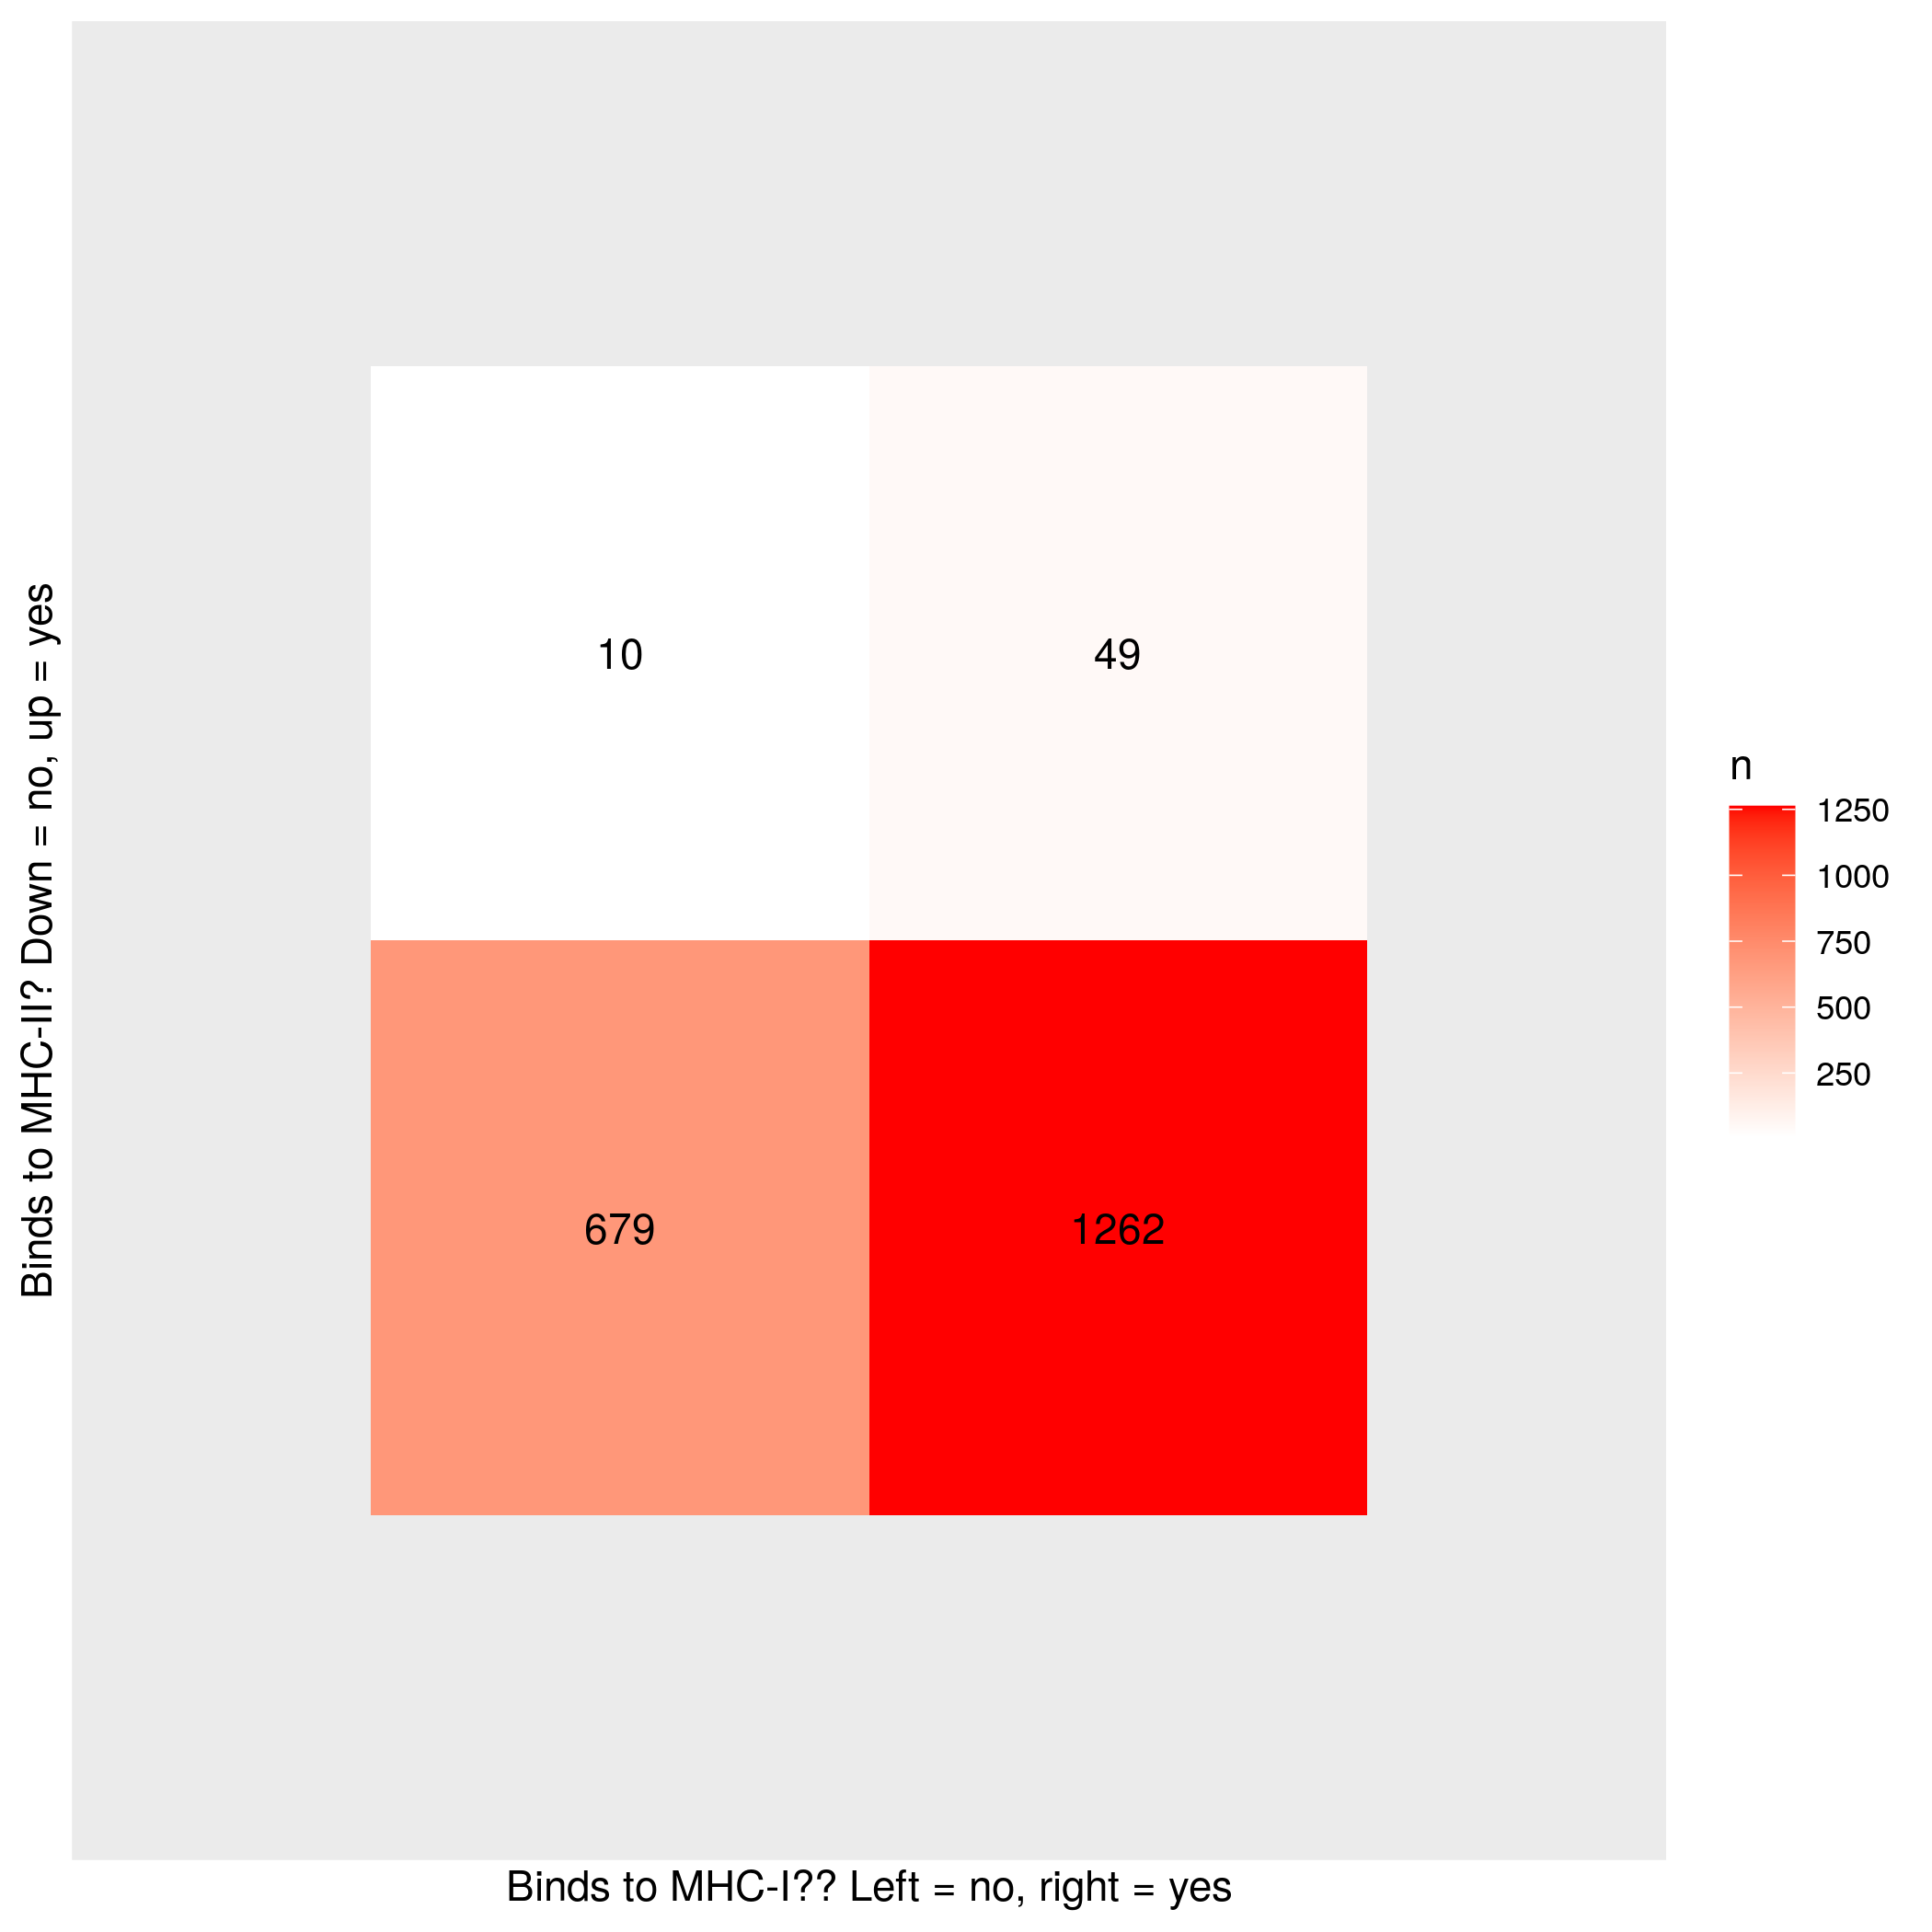
\includegraphics[width=0.9\textwidth]{p_bind_per_hydrophobicity/binds_mhc1_vs_binds_mhc2.png}
  \caption{
    \richel{Used randomly simulated peptides, results are real}
  }
  \label{fig:binds_mhc1_vs_binds_mhc2}
\end{figure}

\begin{figure}[!htbp]
  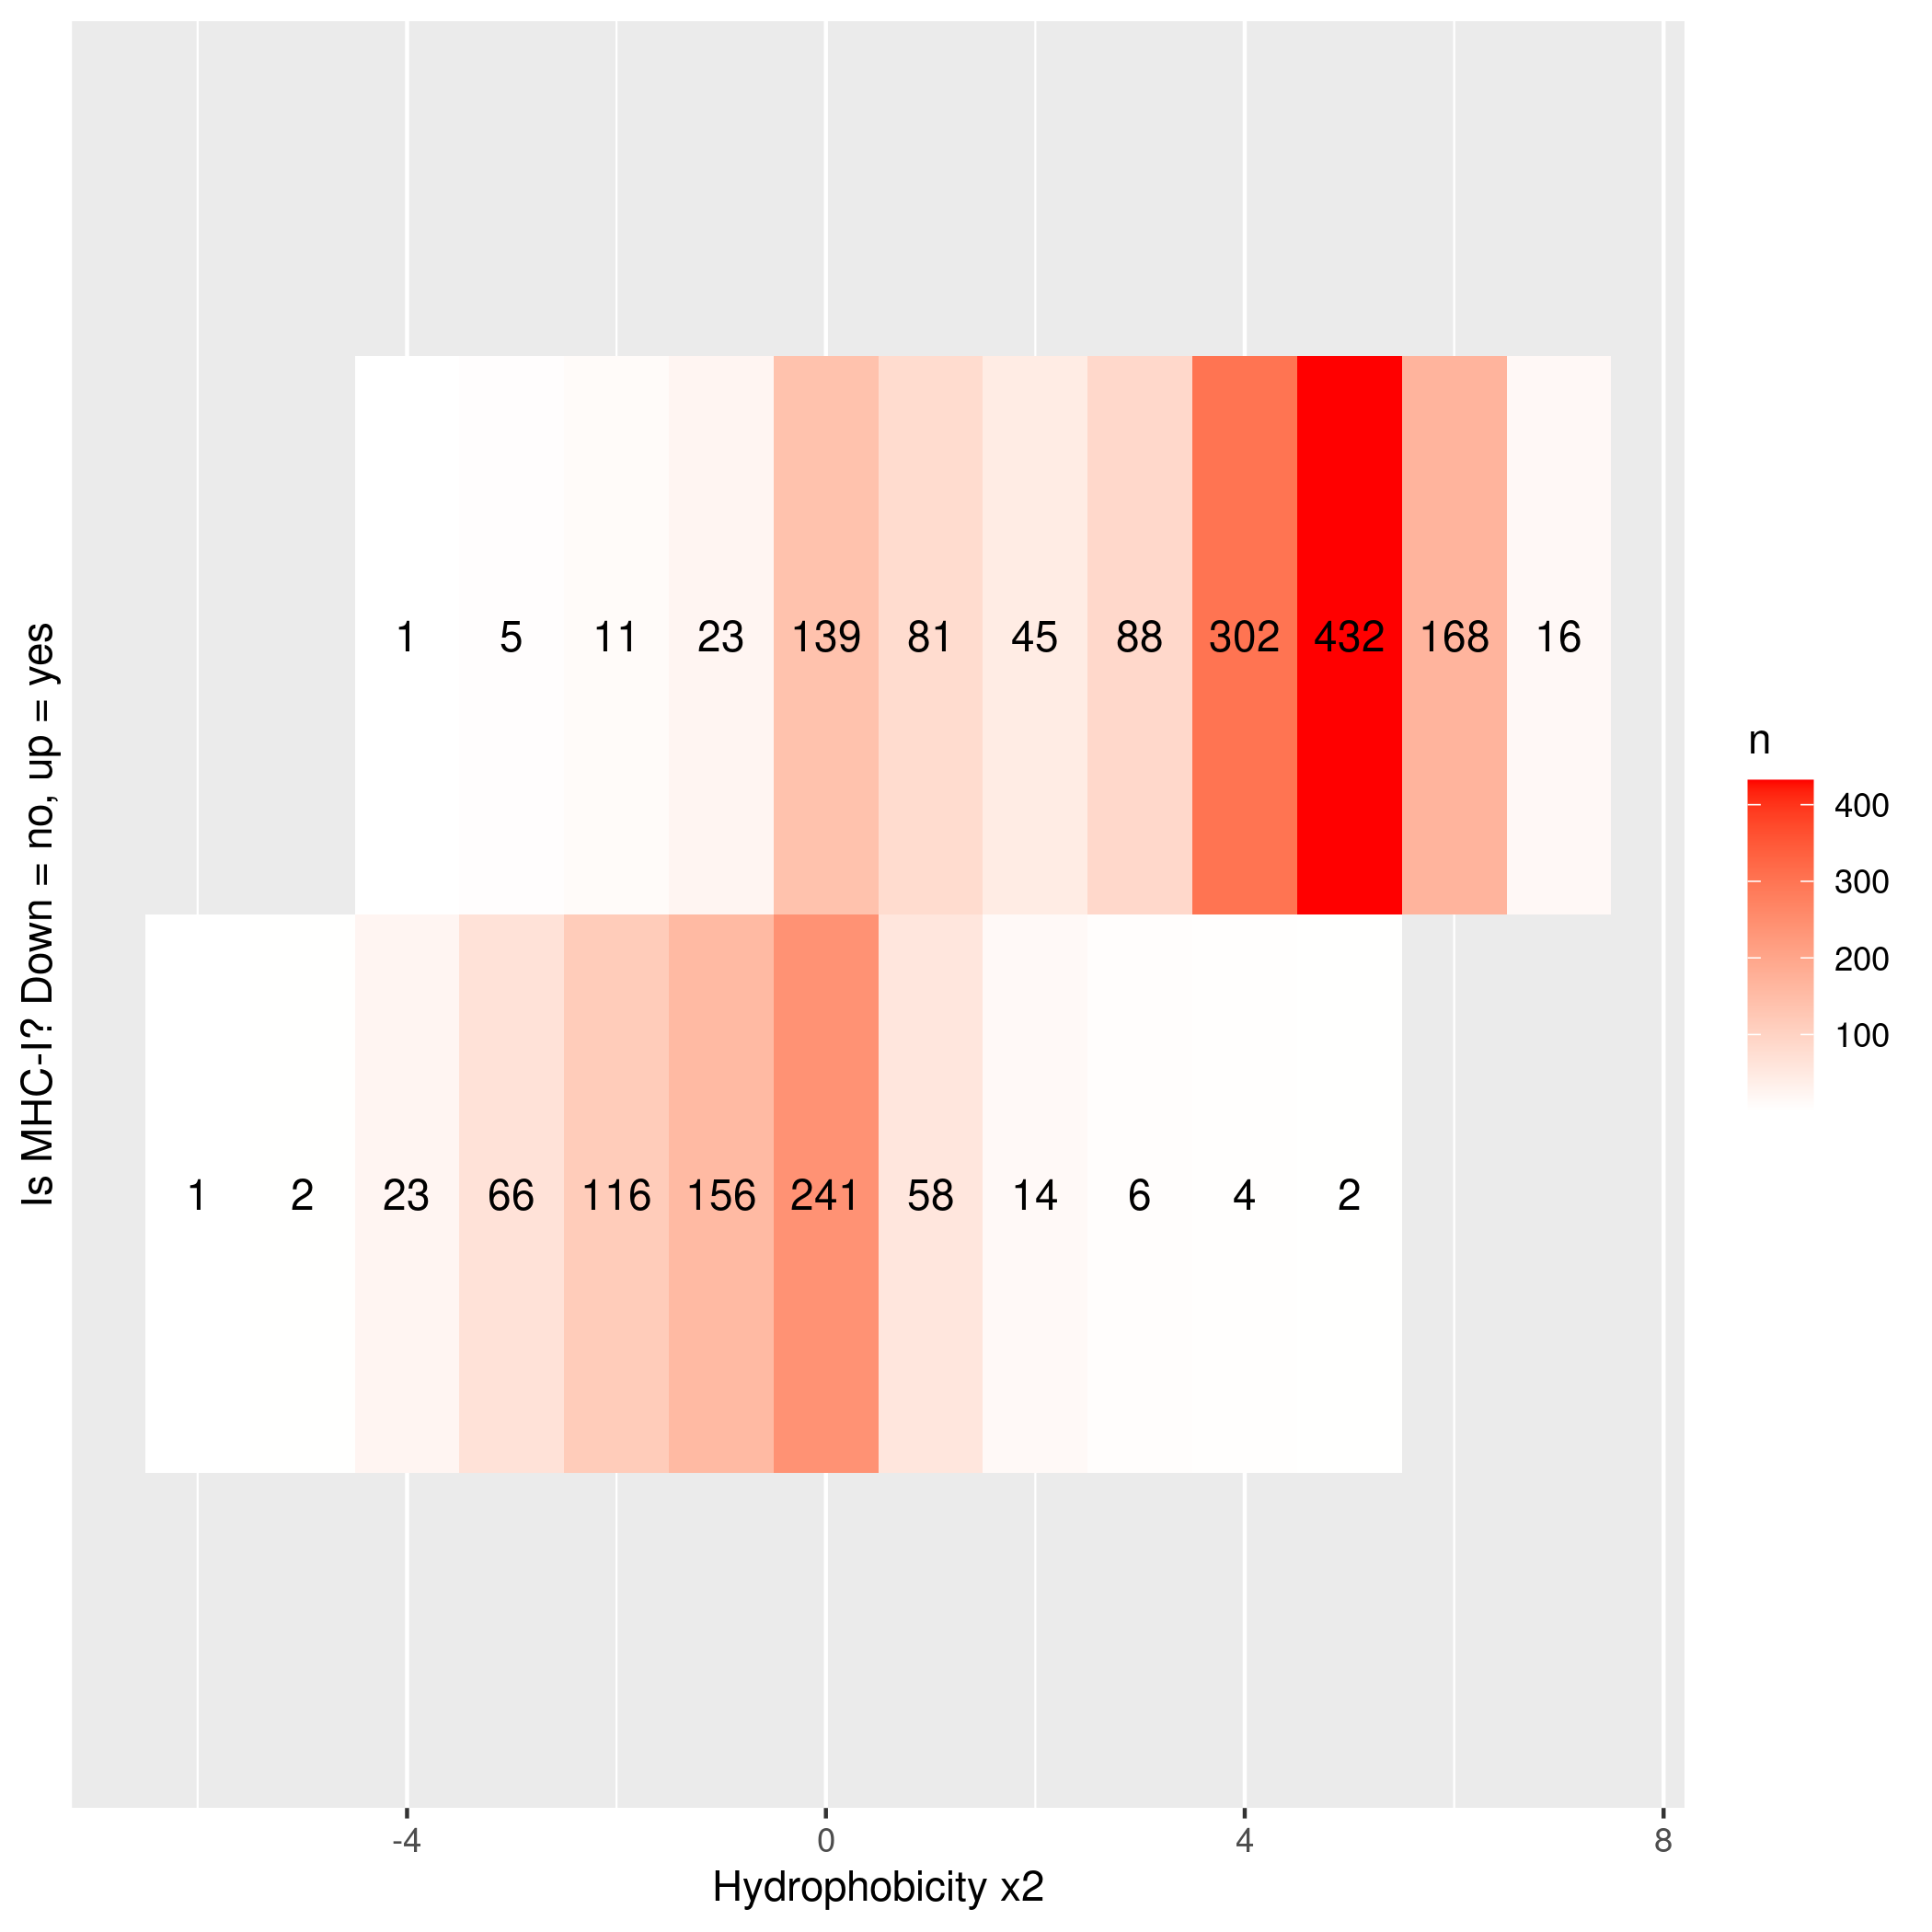
\includegraphics[width=0.9\textwidth]{p_bind_per_hydrophobicity/hydrophobicity_vs_binds_mhc1.png}
  \caption{
    \richel{Used randomly simulated peptides, results are real}
  }
  \label{fig:hydrophobicity_vs_binds_mhc1}
\end{figure}

\begin{figure}[!htbp]
  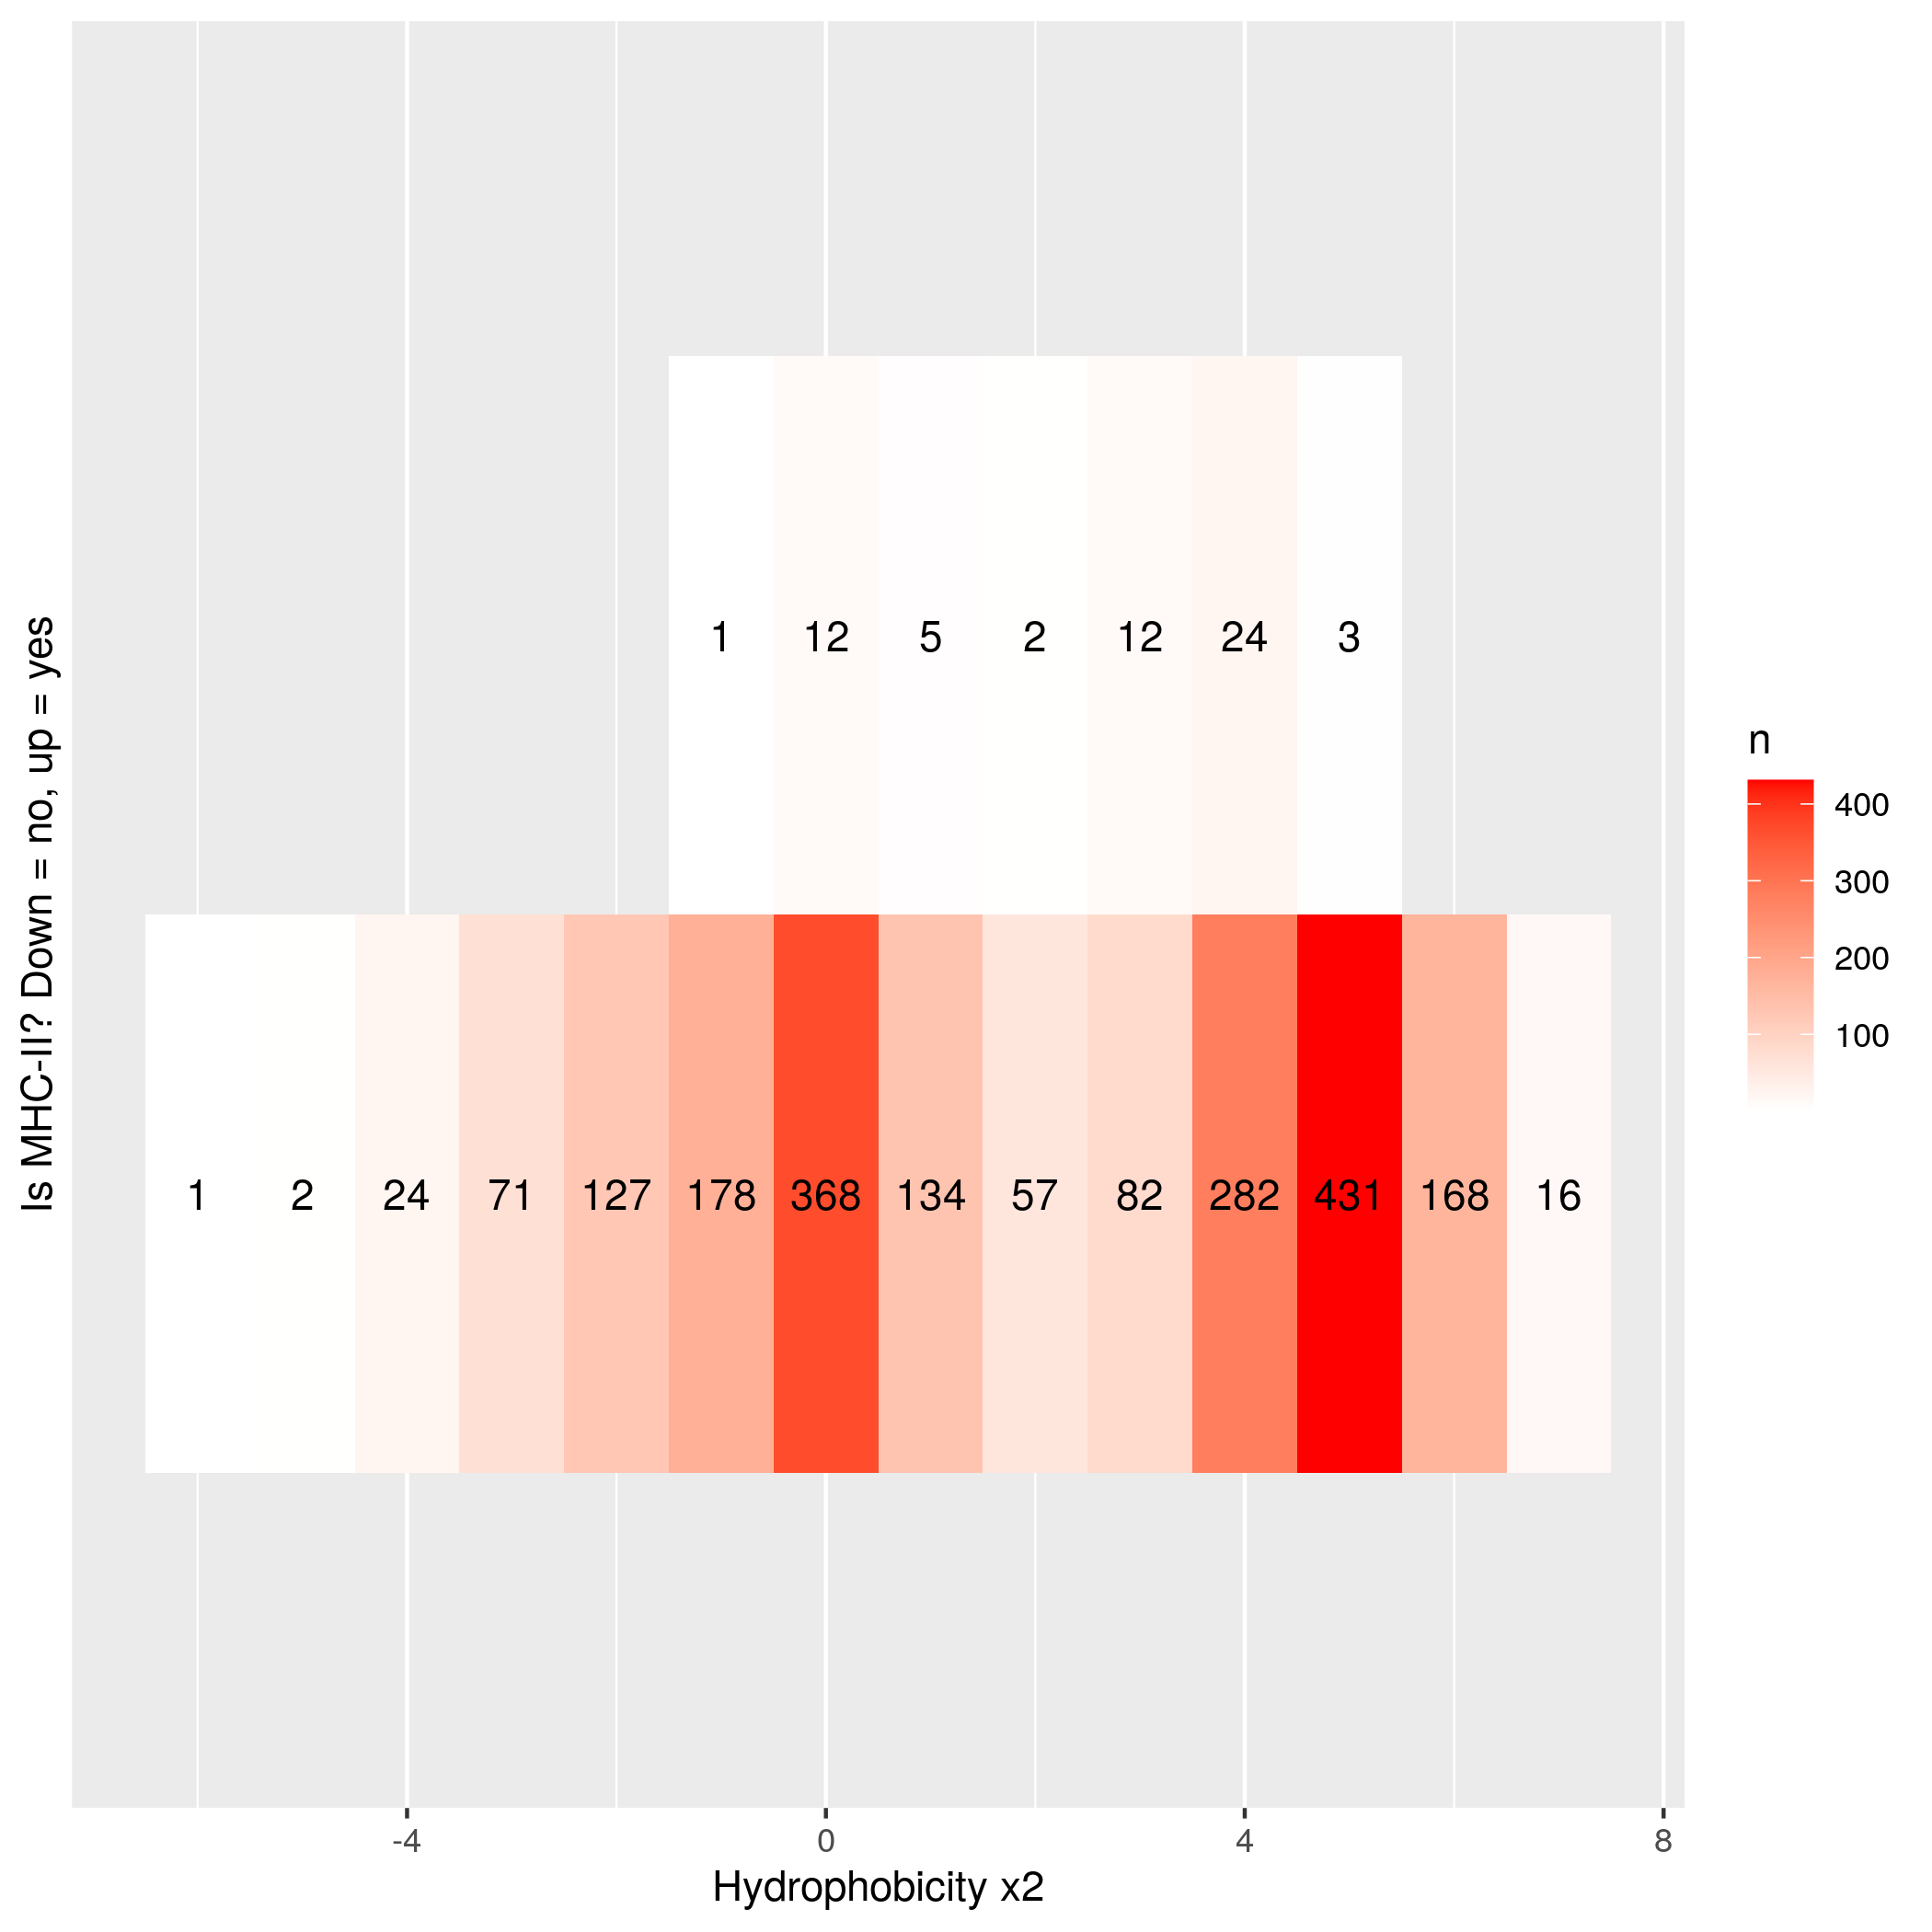
\includegraphics[width=0.9\textwidth]{p_bind_per_hydrophobicity/hydrophobicity_vs_binds_mhc2.png}
  \caption{
    \richel{Used randomly simulated peptides, results are real}
  }
  \label{fig:hydrophobicity_vs_binds_mhc2}
\end{figure}

\begin{figure}[!htbp]
  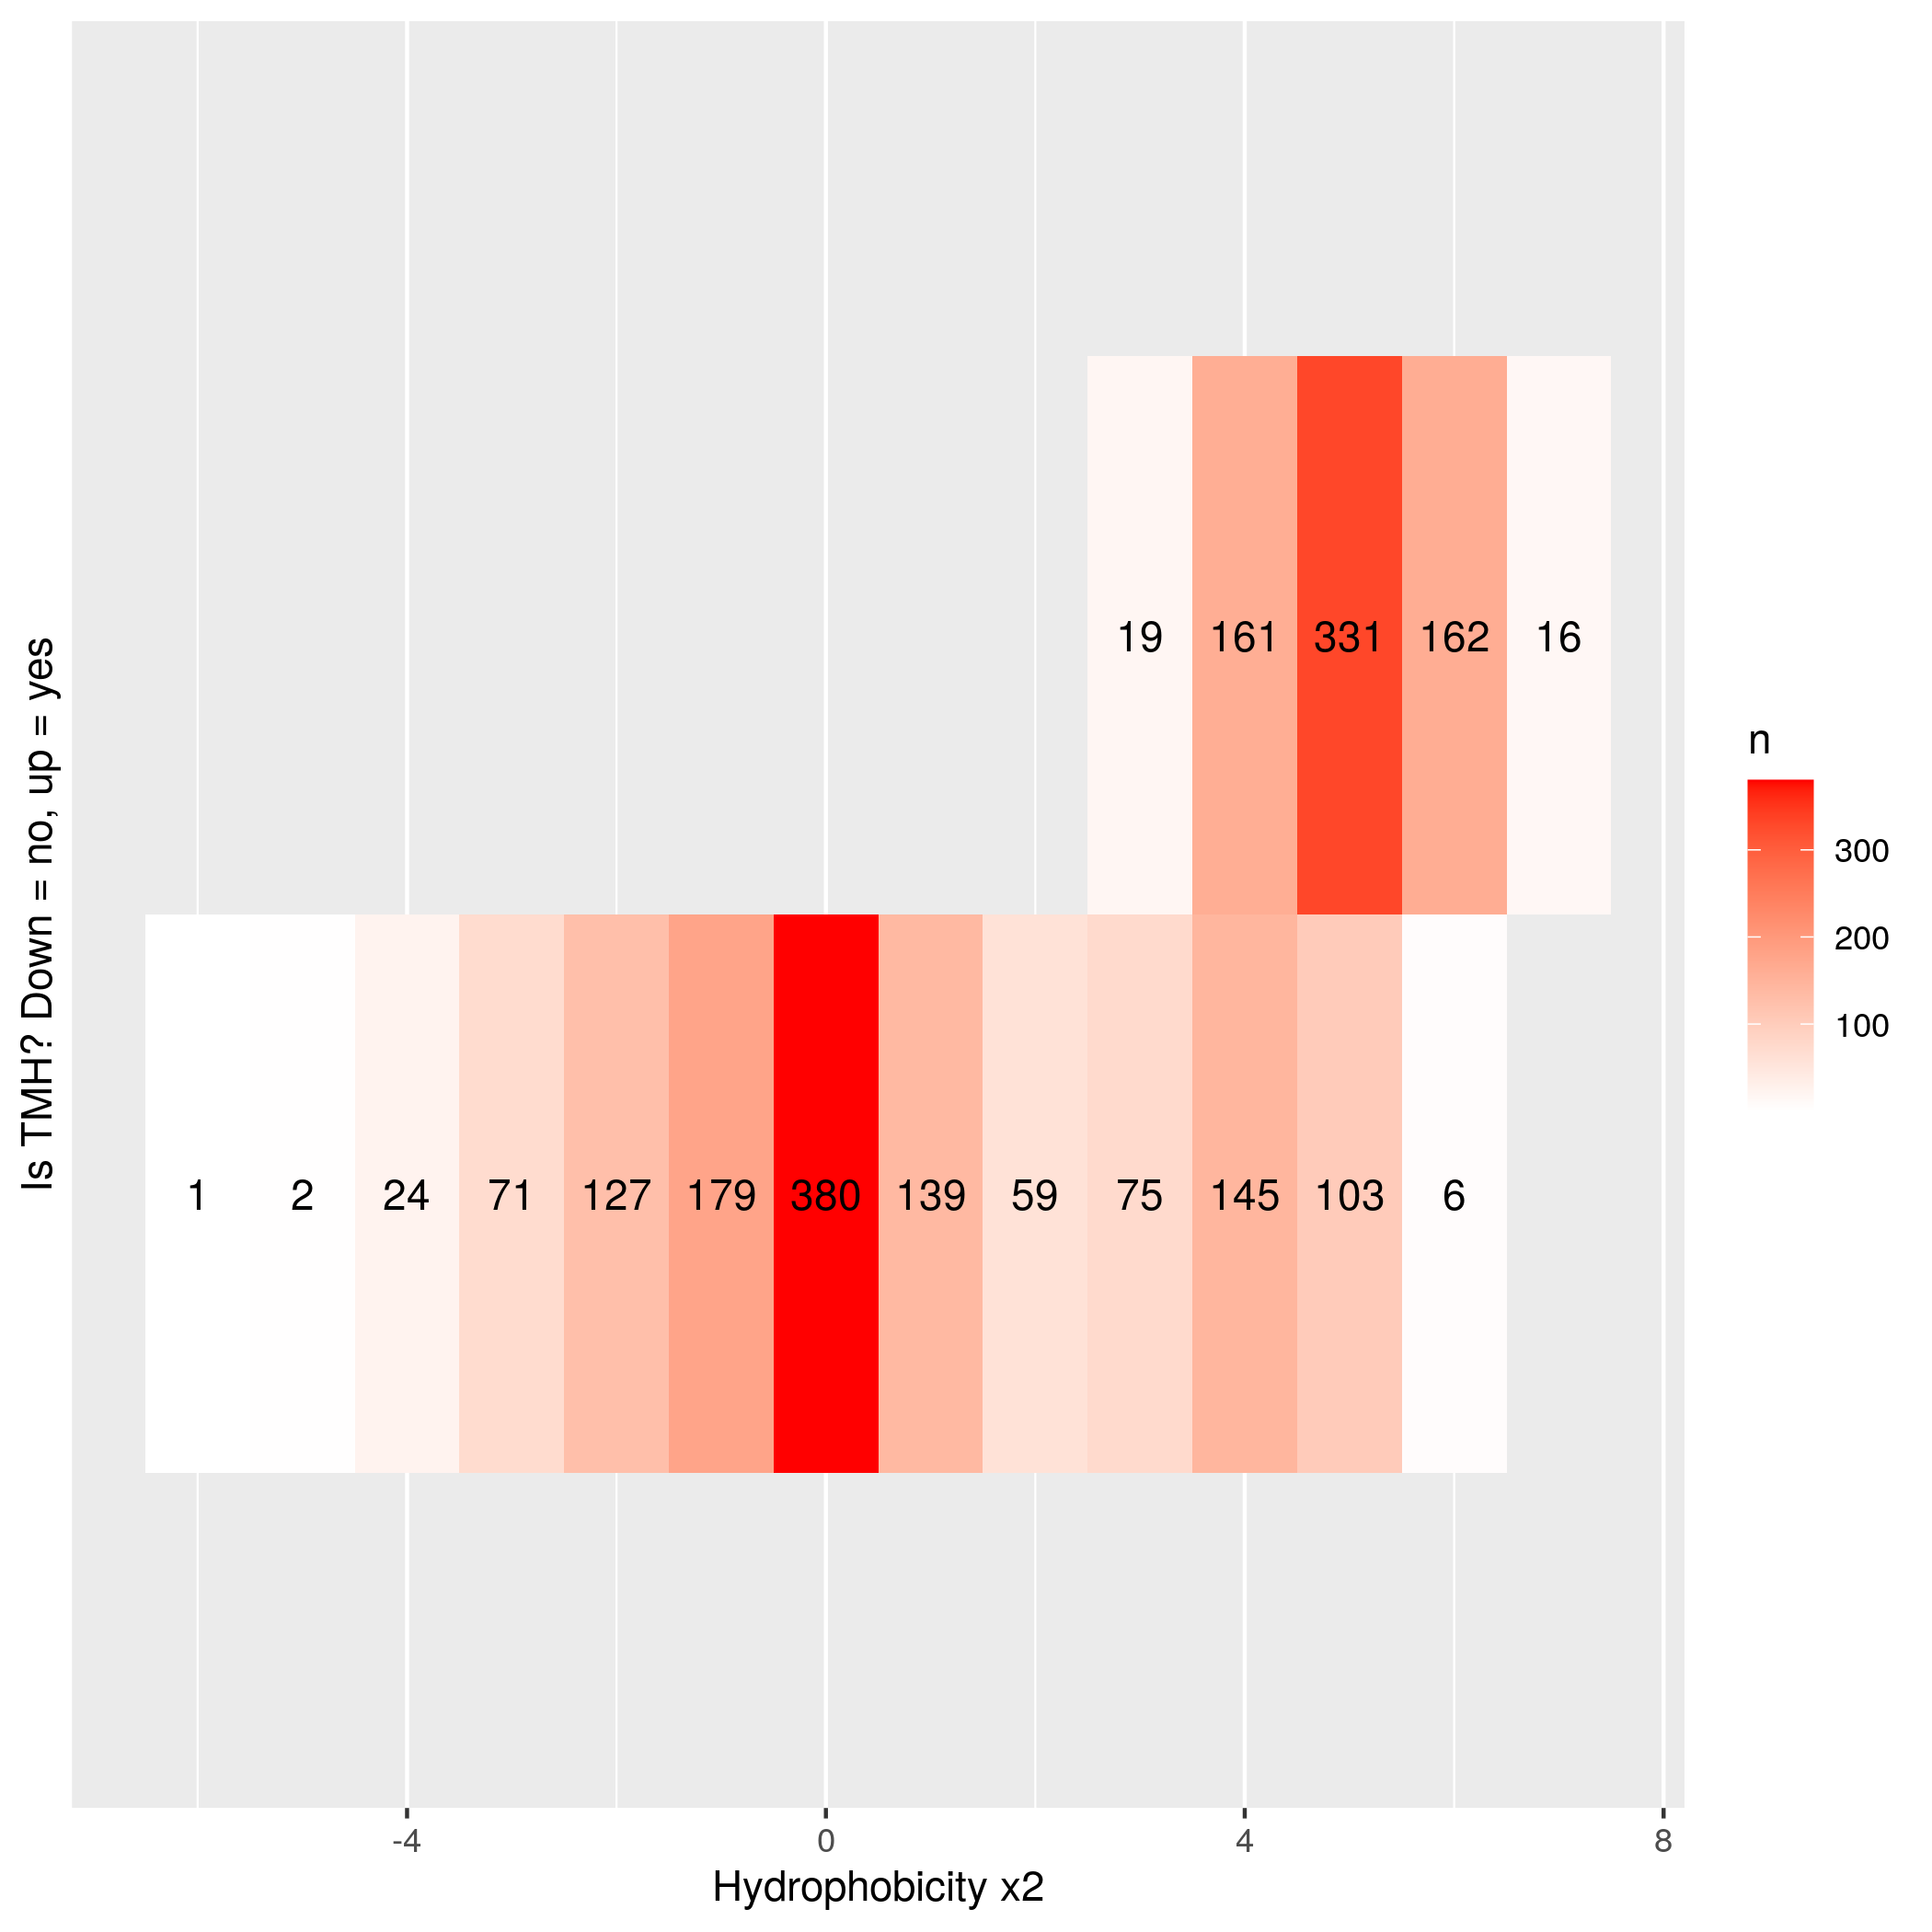
\includegraphics[width=0.9\textwidth]{p_bind_per_hydrophobicity/hydrophobicity_vs_is_tmh.png}
  \caption{
    \richel{Used randomly simulated peptides, results are real}
  }
  \label{fig:hydrophobicity_vs_is_tmh}
\end{figure}

\begin{figure}[!htbp]
  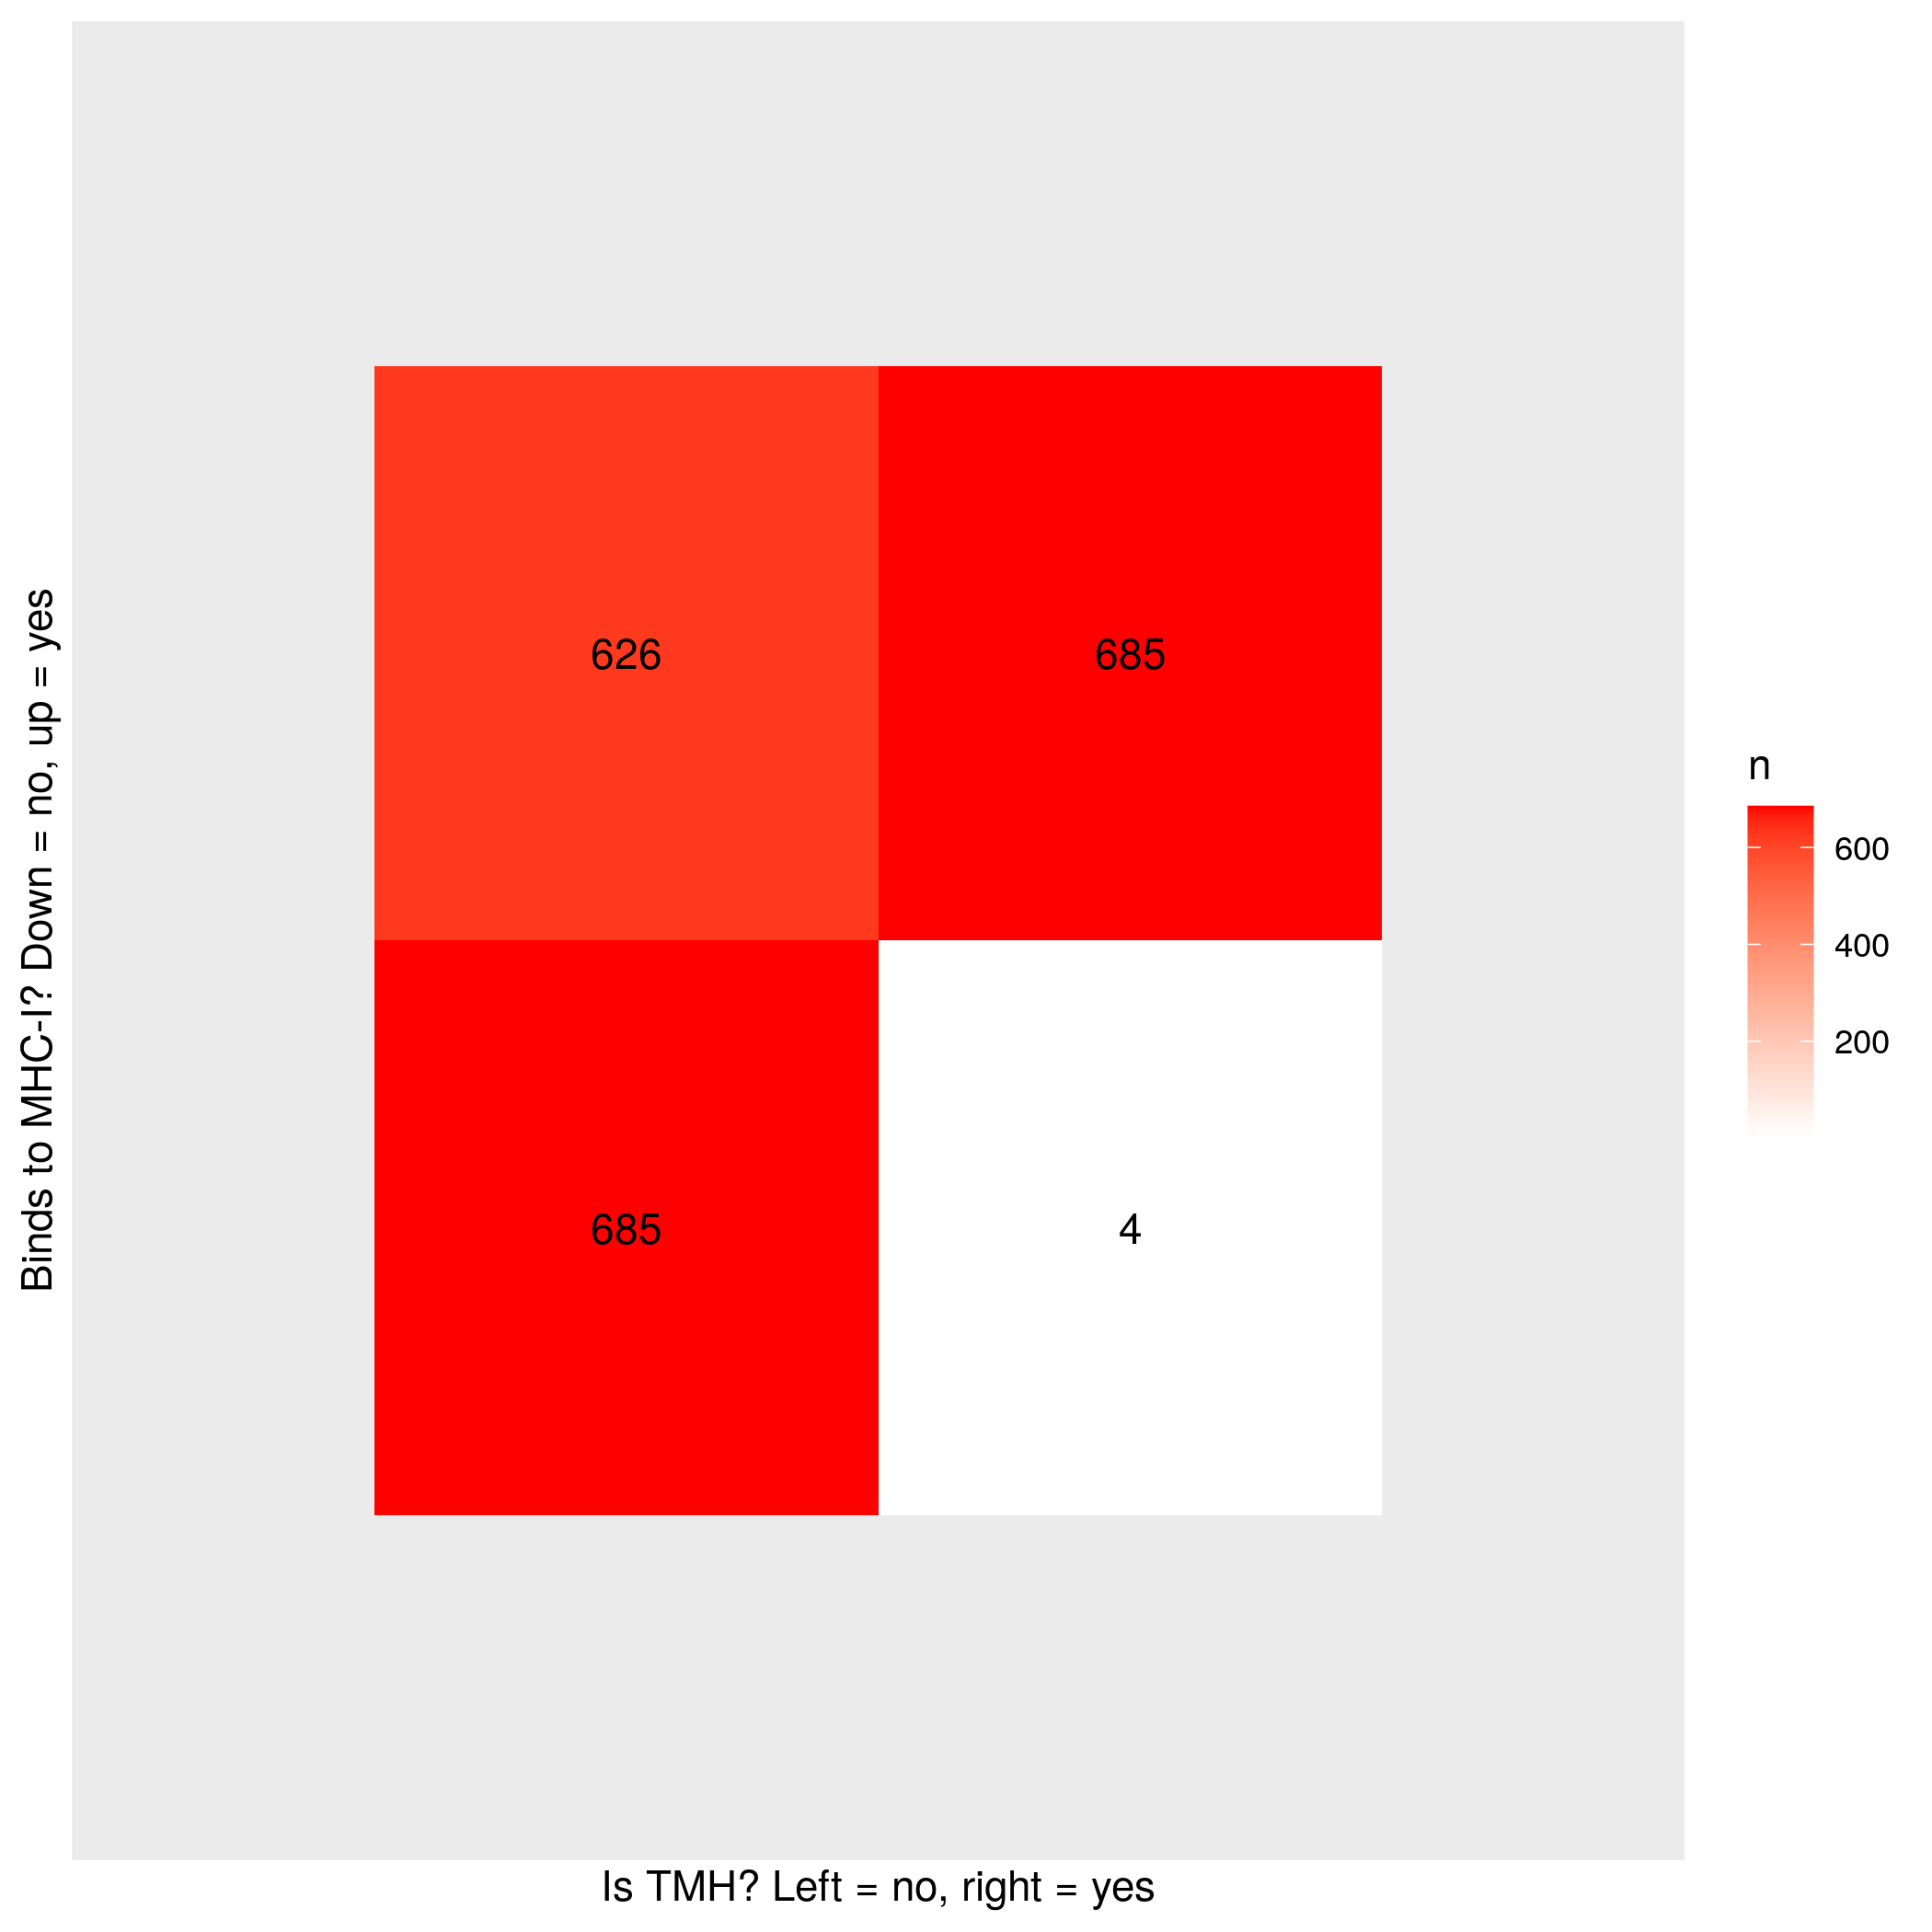
\includegraphics[width=0.9\textwidth]{p_bind_per_hydrophobicity/is_tmh_vs_binds_mhc1.png}
  \caption{
    \richel{Used randomly simulated peptides, results are real}
  }
  \label{fig:is_tmh_vs_binds_mhc1}
\end{figure}

\begin{figure}[!htbp]
  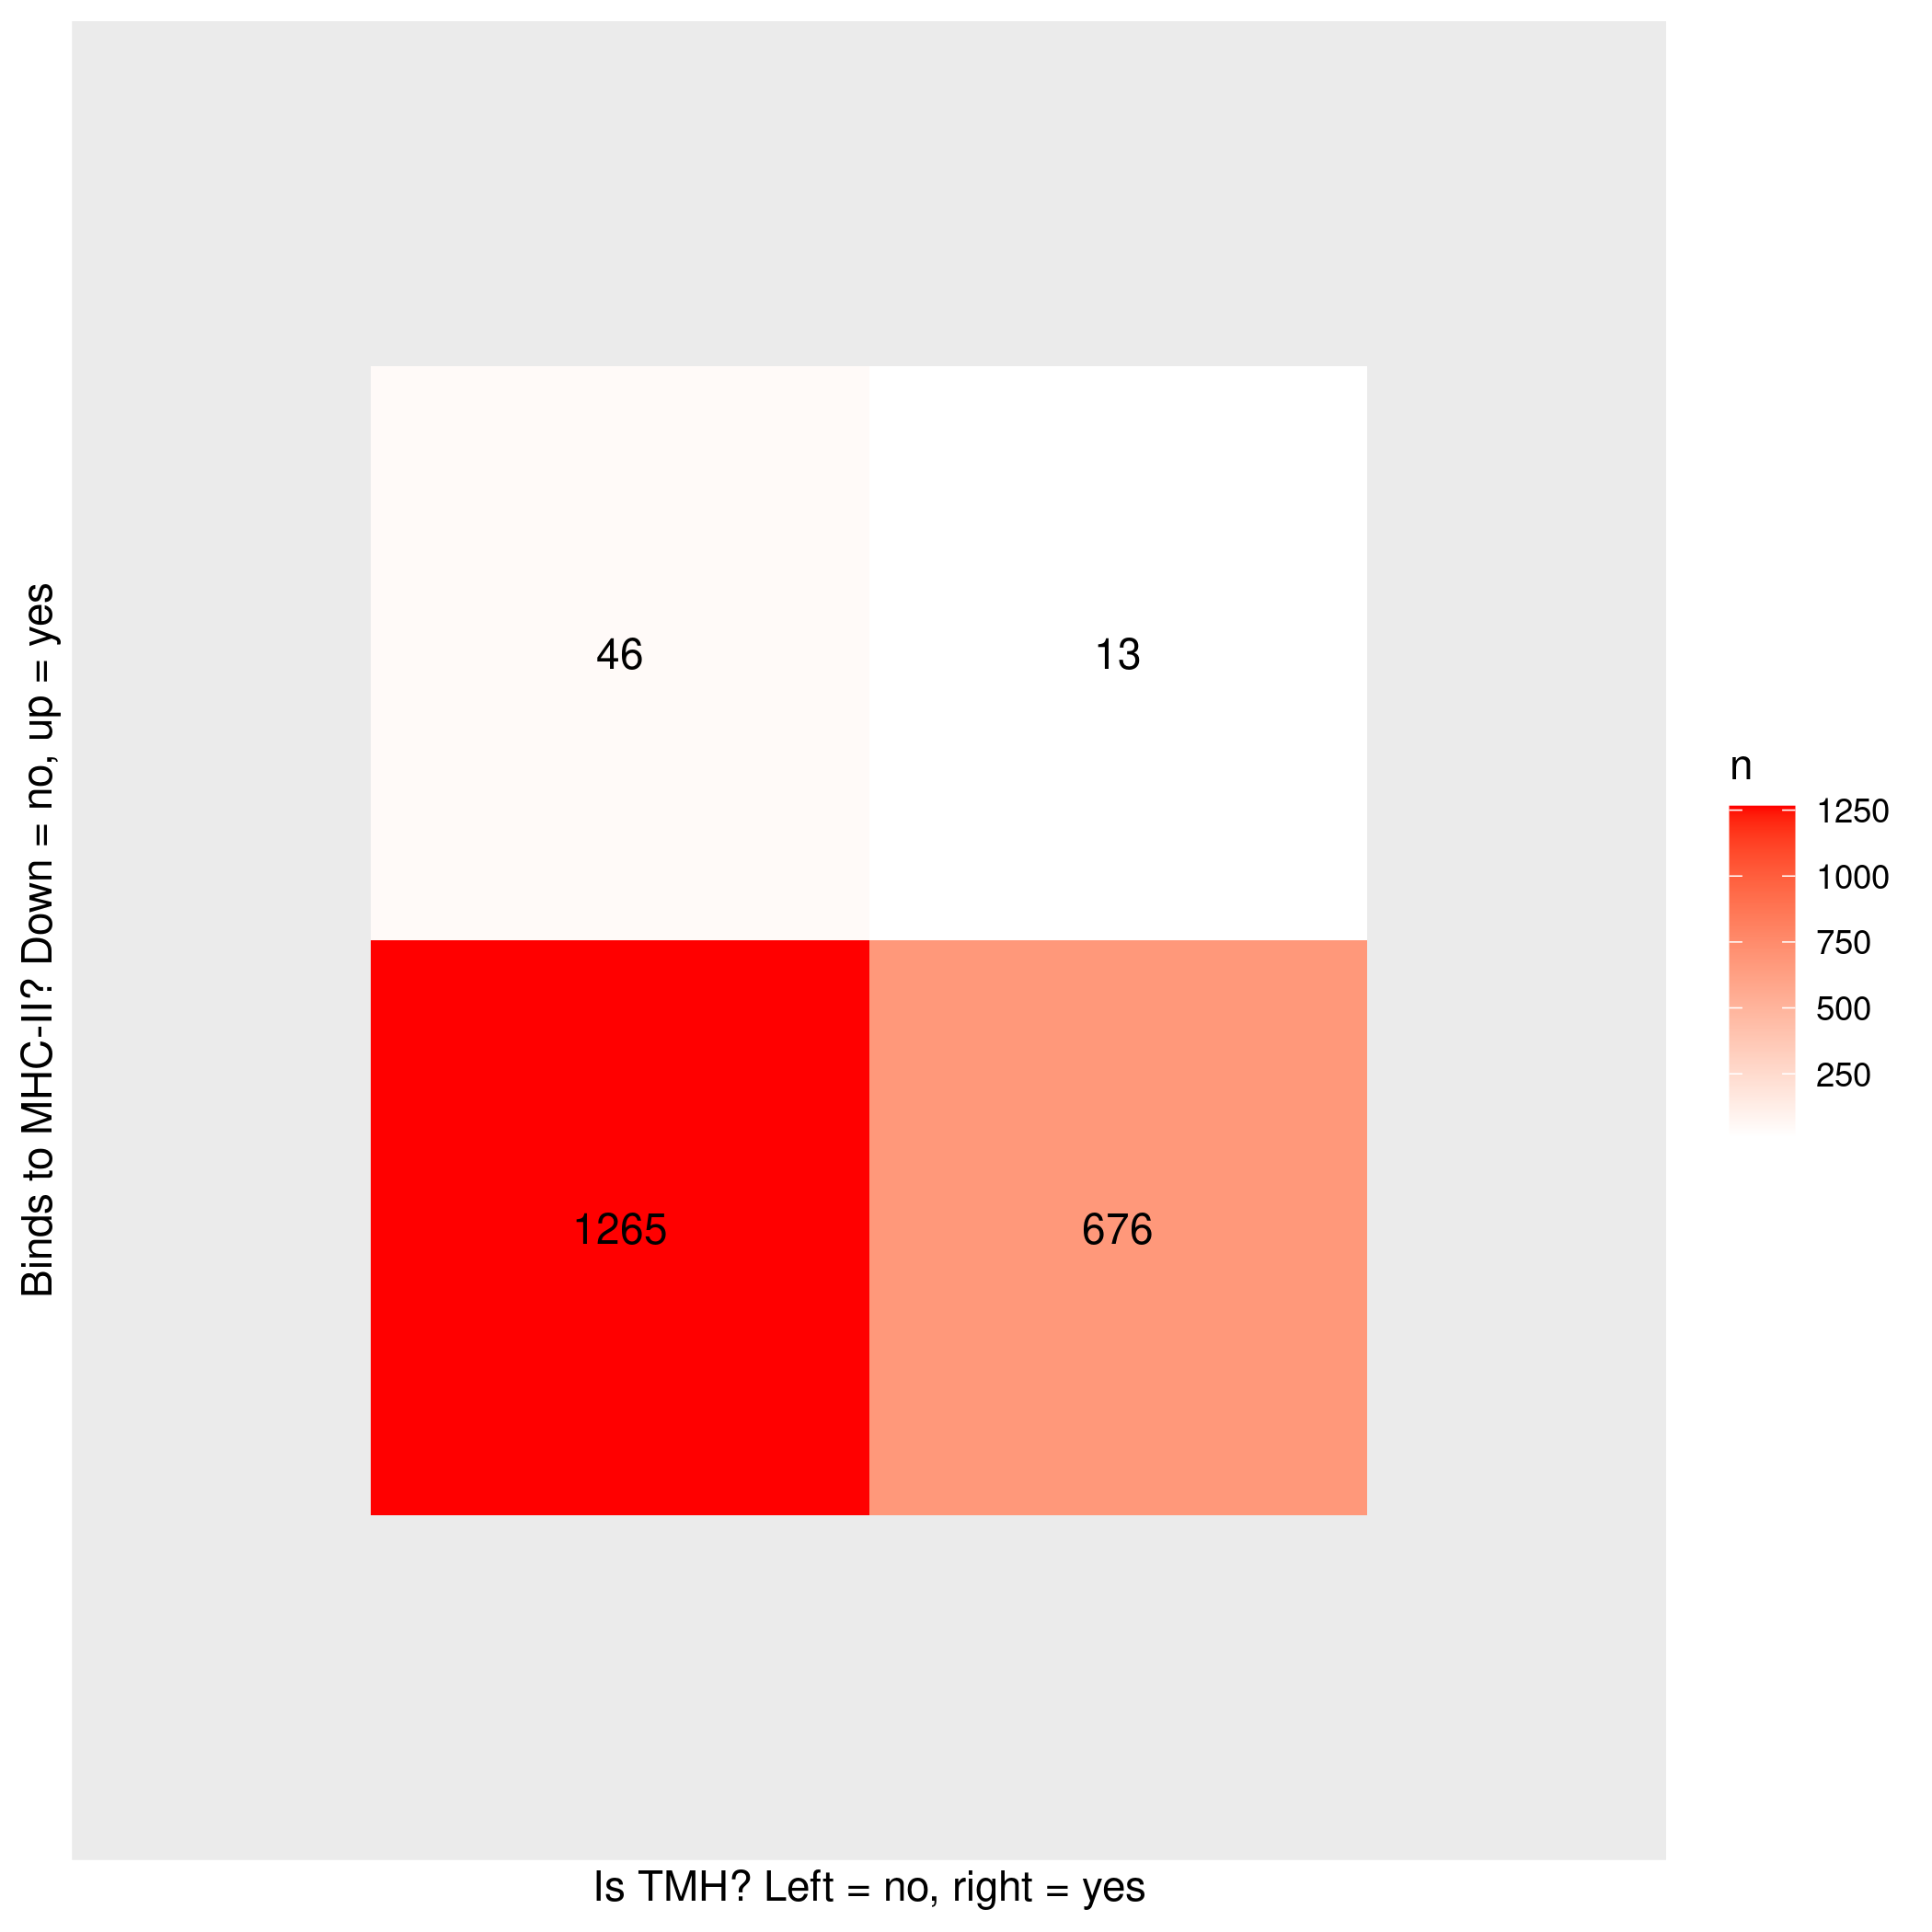
\includegraphics[width=0.9\textwidth]{p_bind_per_hydrophobicity/is_tmh_vs_binds_mhc2.png}
  \caption{
    \richel{Used randomly simulated peptides, results are real}
  }
  \label{fig:is_tmh_vs_binds_mhc2}
\end{figure}


%%%%%%%%%%%%%%%%%%%%%%%%%%%%%%%%%%%%%%%%%%%%%%%%%%%%%%%%%%%%%%%%%%%%%%%%%%%%%%%%
%\subsection{COVID-19 TMHs}
%%%%%%%%%%%%%%%%%%%%%%%%%%%%%%%%%%%%%%%%%%%%%%%%%%%%%%%%%%%%%%%%%%%%%%%%%%%%%%%%

\begin{figure}[!htbp]
  \includegraphics[width=\textwidth]{tmhs/tmhs.png}
  \caption{
    Location of amino acids of reference COVID-19 
    proteome (Uniprot ID: UP000464024).
    Note that ORF1a results in multiple proteins, 
    as shown in figure \ref{fig:covid_genome_and_proteome}.
    Legend: 1 = located in the membrane, 0 = not located in the membrane.
    Topology obtained using 'pureseqtmr' \cite{pureseqtmr}
  }
  \label{fig:covid_topology}
\end{figure}

\begin{table}[!htbp]
  \input{tmhs/covid_tmhs.latex}
  \caption{
    Number of TMHs per COVID-19 ORF,
    using 'pureseqtmr' \cite{pureseqtmr}
  }
  \label{table:covid_tmhs}
\end{table}

%%%%%%%%%%%%%%%%%%%%%%%%%%%%%%%%%%%%%%%%%%%%%%%%%%%%%%%%%%%%%%%%%%%%%%%%%%%%%%%%
\subsection{MHC-II haplotype occurrences}
%%%%%%%%%%%%%%%%%%%%%%%%%%%%%%%%%%%%%%%%%%%%%%%%%%%%%%%%%%%%%%%%%%%%%%%%%%%%%%%%

\richel{
  This is just a reminder, instead of new research. 
  This subsection be deleted in the future.
}

\begin{table}[!htbp]
  \input{mhc2_haplotypes.latex}
  \caption{
    Percentage of MHC-II haplotypes, from \cite{greenbaum2011functional}
    \richel{
      This is just a reminder, instead of new research. 
      This table be deleted in the future.
    }
  }
  \label{table:mhc2_haplotypes}
\end{table}

%%%%%%%%%%%%%%%%%%%%%%%%%%%%%%%%%%%%%%%%%%%%%%%%%%%%%%%%%%%%%%%%%%%%%%%%%%%%%%%%
\subsection{Kolmogorov-Smirnov}
%%%%%%%%%%%%%%%%%%%%%%%%%%%%%%%%%%%%%%%%%%%%%%%%%%%%%%%%%%%%%%%%%%%%%%%%%%%%%%%%

\richel{
  This is just a reminder, instead of new research. 
  This subsection be deleted in the future.
}

The Kolmogorov-Smirnov (KS) test determines if two samples
are derived from the same distribution, without making assumptions
regarding the shape of that distribution. 

We will reject
the null hypothesis that MHC-I has the same percentage of epitopes 
overlapping with TMHs in Homo sapiens compared to each pathogen when 
the KS statistic $D_{n,m}$ follows the relationship as shown in 
equation \ref{eq:ks}, for a significance level $\alpha = 0.05$
and $n = m$ equals the number of HLA haplotypes.

\begin{equation}
   D_{n,m} > \frac{1}{\sqrt{n}} \cdot \sqrt{ -\ln(\frac{\alpha}{2}) \cdot \frac{1 + \frac{n}{m}}{2} }
   \label{eq:ks}
\end{equation}

%%%%%%%%%%%%%%%%%%%%%%%%%%%%%%%%%%%%%%%%%%%%%%%%%%%%%%%%%%%%%%%%%%%%%%%%%%%%%%%%
\subsection{Added PDFs}
%%%%%%%%%%%%%%%%%%%%%%%%%%%%%%%%%%%%%%%%%%%%%%%%%%%%%%%%%%%%%%%%%%%%%%%%%%%%%%%%

These PDFs are added. These will be moved into the article when needed.


